\documentclass[12pt,a4paper]{article} % A4 paper and 11pt font size

\usepackage[utf8x]{inputenc}
\usepackage{braket}
\usepackage{amsmath}
\usepackage{amssymb}
\usepackage{bm}
%\usepackage[utf8]{inputenc}
\usepackage{verbatim}
\usepackage{tikz}
%\usepackage{tikz-feynman}
%\usepackage{pgfornament}
\usepackage{pgfplots}
\usepackage{pgffor}
\usepackage[version-1-compatibility]{siunitx}
\usepackage{fancyhdr}
\usepackage{lipsum}
\usepackage{gensymb}
\usepackage{framed}
\usepackage{cancel}
\usepackage{slashed}
\usepackage{hyperref}
\usepackage{pdflscape}
\usepackage{graphicx}
\usepackage{caption}
\usepackage{subcaption}
\usepackage{geometry}
\usepackage{yfonts}
\usepackage{calc}
\usepackage{cite}

\usepackage{caption}
\usepackage{subcaption}




%%%%%%%%%%%%%%%CATE'S PREAMBLE BIT (TikZ for Feynman diagrams)%%%%%%%%%%%%%%%%

\usepackage{tikz}
\usetikzlibrary{arrows,shapes}
\usetikzlibrary{trees}
\usetikzlibrary{patterns}
\usetikzlibrary{matrix,arrows} 				% For commutative diagram
											% http://www.felixl.de/commu.pdf
\usetikzlibrary{positioning}				% For "above of=" commands
\usetikzlibrary{calc,through}				% For coordinates
\usetikzlibrary{decorations.pathreplacing}  % For curly braces
% http://www.math.ucla.edu/~getreuer/tikz.html
\usepackage{pgffor}							% For repeating patterns

\usetikzlibrary{decorations.pathmorphing}	% For Feynman Diagrams
\usetikzlibrary{decorations.markings}
\tikzset{
	% >=stealth', %%  Uncomment for more conventional arrows
    vector/.style={decorate, decoration={snake}, draw},
	provector/.style={decorate, decoration={snake,amplitude=2.5pt}, draw},
	antivector/.style={decorate, decoration={snake,amplitude=-2.5pt}, draw},
    fermion/.style={draw=black, postaction={decorate},
        decoration={markings,mark=at position .55 with {\arrow[draw=black]{>}}}},
    fermionbar/.style={draw=black, postaction={decorate},
        decoration={markings,mark=at position .55 with {\arrow[draw=black]{<}}}},
    fermionnoarrow/.style={draw=black},
    gluon/.style={decorate, draw=black,
        decoration={coil,amplitude=4pt, segment length=5pt}},
    scalar/.style={dashed,draw=black, postaction={decorate},
        decoration={markings,mark=at position .55 with {\arrow[draw=black]{>}}}},
    neutrino/.style={dashed,draw=black},
    scalarbar/.style={dashed,draw=black, postaction={decorate},
        decoration={markings,mark=at position .55 with {\arrow[draw=black]{<}}}},
    scalarnoarrow/.style={dashed,draw=black},
    electron/.style={draw=black, postaction={decorate},
        decoration={markings,mark=at position .55 with {\arrow[draw=black]{>}}}},
    bigvector/.style={decorate, decoration={snake,amplitude=4pt}, draw},
    arrow/.style={draw=black, postaction={decorate},
        decoration={markings,mark=at position 1 with {\arrow[draw=black]{>}}}},
}

% TIKZ - for block diagrams, 
% from http://www.texample.net/tikz/examples/control-system-principles/
% \usetikzlibrary{shapes,arrows}
\tikzstyle{block} = [draw, rectangle, 
    minimum height=3em, minimum width=6earticlem]

%%%%%%%%%%%%%%END CATE'S PREAMBLE BIT%%%%%%%%%%%%%

\tikzset{>=latex}

\tikzset{cross/.style={cross out, draw, minimum size=2*(#1-\pgflinewidth),
			inner sep=0pt, outer sep=0pt}}
			
\tikzset{snake it/.style={decorate, decoration=snake}}






% Coloured rows in table
\usepackage{color, colortbl}


\setlength{\parindent}{2em}
\setlength{\parskip}{1em}
\newcommand{\goth}[1]{{\Huge\textfrak{#1}}}
\renewcommand{\baselinestretch}{1.1}

\newcommand{\br}{\mathcal{B}}
\newcommand{\tmg}{\tau\to\mu\gamma}
\newcommand{\tlg}{\tau\to\ell\gamma}
\newcommand{\htm}{h\to \tau \mu}

 \geometry{
 a4paper,
 total={210mm,297mm},
 left=28mm,
 right=28mm,
 top=30mm,
 bottom=40mm,
 }


%----------------------------------------------------------------------------------------
%	TITLE SECTION
%----------------------------------------------------------------------------------------
%\setlength\parindent{0pt} % Removes all indentation from paragraphs - comment this line for an assignment with lots of text


\pagenumbering{arabic}
\begin{document}
\pagestyle{empty}

\newcommand{\HRule}{\rule{\linewidth}{0.5mm}}

\begin{titlepage}

    \begin{center}
        %\textsc{\large SN: 587623}
        \vspace*{5cm}

        %\pgfornament[width = 0.9\textwidth, symmetry=v]{88}\\[0.75cm]
        \HRule \\[0.75cm]
		\Huge \textbf{$\bm{\tau\to\ell \gamma}$ at Belle II}\\[0.5cm]
        %\pgfornament[width = 0.9\linewidth]{88}\\[1.5cm]
        \HRule \\[1.5cm]
        \begin{minipage}{0.4\textwidth}
        \begin{center}

        \large By \\[0.75cm]
        \huge Braden \scshape Moore \\[0.5cm]
        \normalsize \normalfont Master of Science \\
        The University of Melbourne \\

        \end{center}
        \end{minipage}

        \vfill

        \large \today
    \end{center}


\newpage
\end{titlepage}
%----------------------------------------------------------------------------------------
\pagestyle{empty}
\tableofcontents
\newpage

\pagestyle{fancy}
\pagenumbering{arabic}
\rhead{\textsc{Thesis: $\tlg$}}
\setcounter{page}{1}


\section{Lepton Flavour Violation and the Standard Model}

\subsection{Introduction}

Lepton flavour violation (LFV) is an exciting field of research at the frontier of particle physics. Searches for LFV can probe a wide variety of new physics (NP) scenarios. We will not be looking at all LFV; in this literature review we specifically cover charged LFV of the form $\tlg$. Of the tau processes, these modes are predicted to be the most sensitive to NP. We choose to investigate tau LFV rather than, say, muon LFV, for two main reasons. Firstly, the tau processes have predicted branching fractions of $\sim 5 - 6$ orders of magnitude greater than the analogous muon processes, due to the differences in mass \cite{Paradisi:2016}. The decay $\tmg$ has a predicted branching fraction $\sim 6$ orders of magnitude greater than the analogous $\mu\to e \gamma$! Secondly, if this NP introduces Higgs-like particles, we would observe the NP more strongly in the tau sector, since taus couple more strongly to Higgs than do muons.


\begin{figure}[h]
\centering
%\includegraphics[width=0.6\textwidth]{images/taumugamma.png}
\caption{Diagram of $\tmg$ in the Standard Model}
\label{}
\end{figure}

\subsection{LFV and the Standard Model}

LFV necessarily requires generation mixing between leptons to occur. Though this is prohibited in the Standard Model, the discovery of neutrino oscillations proves that flavour mixing does occur in our universe; that is, flavour is not conserved. We seek to discover whether this LFV can be observed in other areas of flavour physics.

In the Standard Model + massive neutrinos, the only source of LFV is from the operators responsible for neutrino mass. However, the relevant Feynman diagrams (see Figure) are ``loop suppressed'' and proportional to the GIM factor, given as $\left(\frac{m_\nu}{M_W}\right)^4$; as neutrino mass is very small ($\mathcal{O}(\SI{0.3}{eV})$) we expect the LFV effects to be negligible! With these operators the branching ratio for, say, $\tmg$ is $\sim 10^{-40}$ \cite{Passemar:2015}. With such little SM background, observation of an LFV process of the type $\tlg$ would be an unambiguous signature of NP.

\begin{equation}
\mathcal{B}(\tau\to\ell\gamma)=\frac{3\alpha}{32\pi}\lvert U^{\star}_{\tau i} U_{\mu i}\frac{\Delta^2_{3i}}{m_W^2}\rvert^2
\leq 10^{-53}\sim 10^{-49}
\end{equation}


\subsection{Other LFV}

In many NP models, LFV is not limited to just $\tlg$ decays. There have been searches for other LFV modes, such as $\mu\to e \gamma$, and $\tau\to 3\ell$. Current limits on the branching fractions are given in Figure \ref{tab:current lfv bounds} below \cite{Paradisi:2016}.

\begin{table}[h]
\centering
\label{my-label}
\begin{tabular}{lll}
\textbf{LFV process} & \textbf{Present bound} & \textbf{Future sensitivity} \\ \hline
$\mu\to e\gamma$ & \num{5.7e-13} & $\approx\num{6e-14}$ \\
$\mu\to 3e$ & \num{1.0e-12} & $\approx\num{e-16}$ \\
$\tau\to e\gamma$ & \num{3.3e-9} & $\sim\num{e-8} - \num{e-9}$ \\
$\tau\to\mu\gamma$ & \num{4.4e-9} & $\sim\num{e-8} - \num{e-9}$ \\
$\tau\to 3e$ & \num{2.7e-8} & $\sim\num{e-9} - \num{e-10}$ \\
$\tau\to 3\mu$ & \num{2.1e-8} & $\sim\num{e-9} - \num{e-10}$
\end{tabular}
\caption{Current experimental limits on various LFV processes}
\label{tab:current lfv bounds}
\end{table}

Moving into future sensitivities accessible from experiments such as Belle II, we see that the upper limits of branching fractions for $\tlg$ decays could be improved by $1-2$ orders of magnitude!

\subsection{Hints of LFV beyond the Standard Model}

Motivations behind the search for LFV come from both theoretical and experimental results. The primary experimental motivations is the existence of neutrino mixing, though anomalous results such as the $\htm$ excess observed at CMS in 2015 also hint at LFV beyond the Standard Model. On the theoretical side, LFV is predicted in a variety of NP models. In fact, many models which introduce mechanisms to generate neutrino mass also inadvertantly allow LFV in other sectors of non-negligible order! We shall discuss these motivations below.


\subsubsection{Neutrino mixing}

The discovery that flavour mixing can occur in the neutrino sector \cite{SuperK:1998}\cite{SNO:2002} proves that neutrinos have mass. Both the concept of massive neutrinos, and by extension the mechanisms which generate neutrino mass, are not predicted or explained by the SM. This tells us that the lepton sector is not fully understood.

There are many NP models which introduce mechanisms to give neutrinos mass. These include SUSY, seesaw models, and many others. In introducing these mechanisms, many of these models inadvertently introduce LFV! As a particle example, a Type-II seesaw model posits a scalar triplet of Higgs-like particles \cite{Passemar:2015}. This triplet comprises a doubly-charged Higgs, a singly-charged Higgs, and a neutral Higgs. As show in Figure X below, lepton-flavour violating processes could proceed via leptons coupling to these scalars!


\begin{figure}[h]
\centering
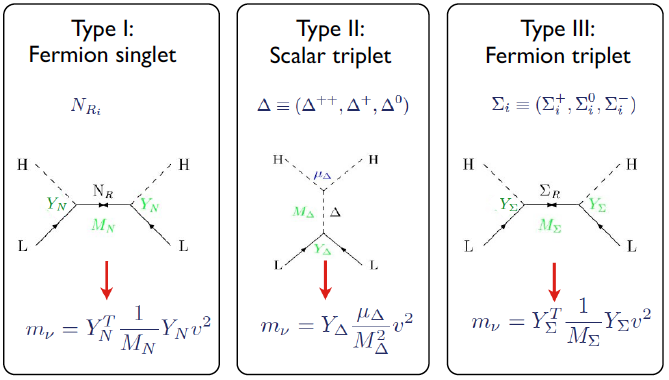
\includegraphics[width=0.7\textwidth]{images/seesaw.png}
\caption{New particles introduced in seesaw models (Passemar, 2015)}
\label{}
\end{figure}

\begin{figure}[h]
\centering
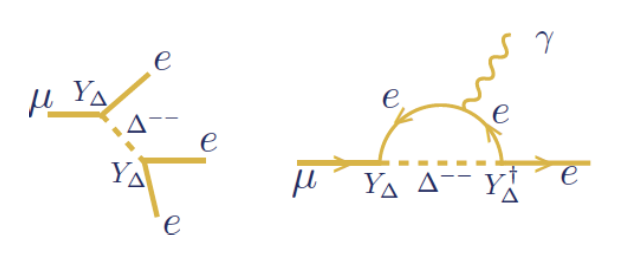
\includegraphics[width=0.5\textwidth]{images/seesaw-lfv-modes.png}
\caption{Scalars introduced in Type-II seesaw models mediating LFV decays (Passemar, 2015)}
\label{}
\end{figure}




\subsubsection{$\htm$ excess}

Hints of LFV can come in the form of experimental results which are not consistent with the SM. One such ``anomaly’’ is the $\htm$ excess. In 2015, CMS found a $2.4\sigma$ excess in the branching fraction of $\htm$ \cite{CMS:2015a}. This process is lepton flavour violating, so in the SM its branching fraction is expected to be consistent with zero. However it was determined

\begin{equation}
\br(h\to \tau \mu) = (0.84^{+0.39}_{-0.37})\%
\end{equation}


Also in 2015 was a similar search performed by ATLAS \cite{ATLAS:2015}, in which an excess of $1.2\sigma$ was found in the $\htm$ decay. 

\begin{equation}
B(\htm) = (0.77 \pm 0.66)\%
\end{equation}

Though this $1.2\sigma$ result is less indicative of NP, it still provides hints as to where NP could occur. These results indicate possible new physics in the Higgs sector! Several models, including Two-Higgs Doublet Models (2HDM), introduce new Higgs-like particles; these particles can couple with leptons to allow lepton flavour violating processes \cite{Harnik:2012}. In fact, LFV can occur naturally in any model with more than one Higgs doublet.


\begin{figure}[h]
\centering
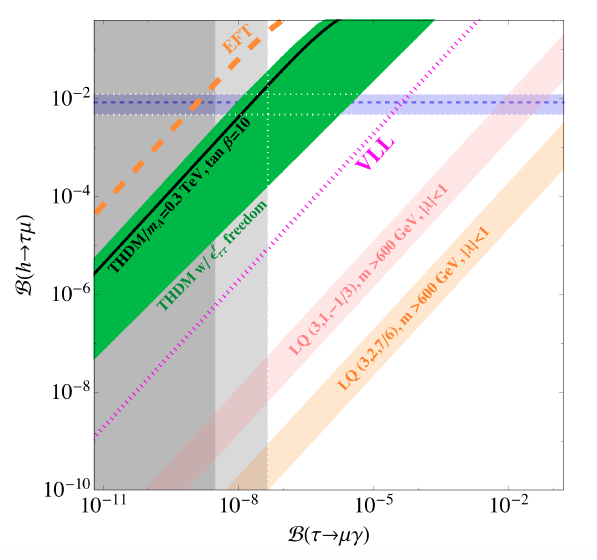
\includegraphics[width=0.7\textwidth]{images/h-vs-tau.png}
\caption{Correlation between $\br(\htm)$ and $\br(\tmg)$ in various NP scenarios (Dorsner et al., 2015)}
\label{}
\end{figure}


The present experimental result for $\br(\htm)$ is shown in horizontal blue band; current and future projections for $\br(\tmg)$ experimental sensitivity are represented with vertical light and dark gray bands. We note that certain 2HDM models predict a branching fraction for $\br(\tmg)$, consistent with the CMS results, at sensitivities which could be observed by Belle II. It is important to note that the Higgs sector could contribute to LFV in NP scenarios, and that both theory and experimental limits on other LFV processes such as $\htm$ all interweave with limits on $\tlg$ branching fractions to provide information on NP, even just through reducing the available phase space for certain models \cite{Dorsner:2015}.

\begin{figure}[h]
\centering
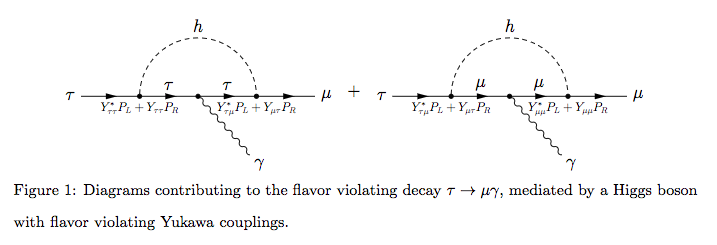
\includegraphics[width=0.9\textwidth]{images/higgs-lfv-modes.png}
\caption{Diagrams contributing to $\tmg$ decay, mediated by a Higgs boson with flavour violating Yukawa coupling (Harnick et al., 2012)}
\label{}
\end{figure}

As seen in Figure above, new Higgs particles can mediate LFV processes and allow for measurable amounts of LFV beyond the Standard Model \cite{Dorsner:2015}.


\subsubsection{Models predicting $\tlg$}

As mentioned previously, LFV in the $\tau$ sector is introduced in many NP scenarios as a consequence of generating neutrino mass (and hence facilitating neutrino mixing). Branching fractions of the modes $\tlg$ are highly calculable - there is little theoretical uncertainty.

\begin{figure}[h]
\centering
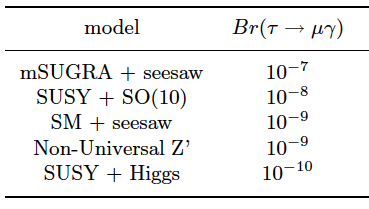
\includegraphics[width=0.5\textwidth]{images/np-models-bounds.png}
\caption{Upper limits of branching fractions from $\tmg$, predicted by models of new physics beyond the SM (various sources)\cite{Ohshima:2007zz}}
\label{}
\end{figure}

Figure above lists a few NP models with their predictions of $\br(\tmg)$. We see that the phase space of some of these models has already been ruled out with our current experimental limits on LFV branching fractions.



\subsection{Searches for $\tlg$}

The most recent searches for $\tlg$ were undertaken at Belle (2007) and Babar (2010), for both $\ell=\mu,e$ modes. These detectors are $e^+ e^-$ colliders; a signal of the form $e^+ e^-\to \tau^+ \tau^-$, with one tau (signal-side) decaying $\tau\to \ell \gamma$ and the other tau (tag-side) decaying generically, with the requirement that the tag-side track is not $\ell$.

The dominant backgrounds for the process $\tmg$ are $\tau\to \mu \nu \nu$, $\tau\to \pi \nu$ and $e^+ e^- \to \mu^+ \mu^- \gamma$ (with similar backgrounds for $\tau\to e \gamma$) \cite{Hayasaka:2007}. The first two backgrounds have branching fractions
\begin{align}
\br(\tau\to \mu \nu \nu)&=17.41\%\\
\br(\tau\to\pi\nu)&=10.83\%
\end{align}
which are non-negligible contributions to the dataset. The cross-section for we can compare the cross section of $e^+ e^- \to \mu^+ \mu^- \gamma$ to that of $e^+ e^- \to \tau^+ \tau^- \gamma$;
\begin{align}
\sigma(e^+ e^- \to \mu^+ \mu^- \gamma)&=\SI{0.242}{nb}\\
\sigma(e^+ e^- \to \tau^+ \tau^- \gamma)&=\SI{0.919}{nb}\\
\end{align}
so we note a significant contribution from this background also.

\begin{figure}[h]
\centering
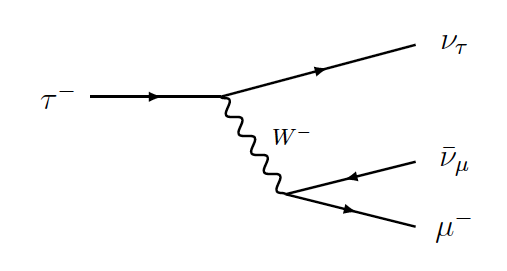
\includegraphics[width=0.3\textwidth]{images/taumununu.png}
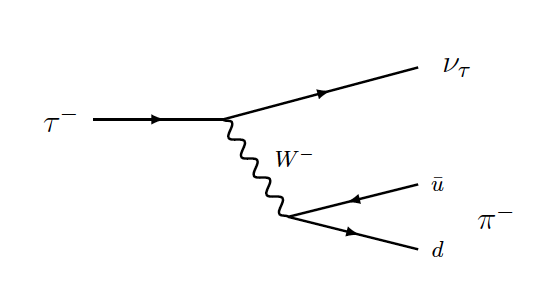
\includegraphics[width=0.3\textwidth]{images/taupinu.png}
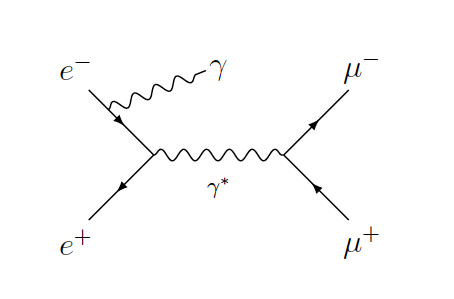
\includegraphics[width=0.3\textwidth]{images/eemumugamma.png}
\caption{Dominant backgrounds to $\tmg$. From left-to-right: $\tau\to \mu \nu \nu$, $\tau\to \pi \nu$ and $e^+ e^- \to \mu^+ \mu^- \gamma$}
\end{figure}


\subsubsection{Belle searches}


The Belle detector records events from an asymmetric $e^+ e^-$ collider with electron (positron) energy of $\SI{8}{GeV}$ ($\SI{3.5}{GeV}$). A detailed discussion of the detector can be found at Ref. \cite{Belle:2002}. In 2007, the Belle Collaboration performed a search over $\SI{535}{fb^{-1}}$ of $e^+ e^-$ data and set constraints \cite{Hayasaka:2007} on $\tlg$ branching fractions as

\begin{align}
\br(\tmg)&<\num{4.5d-8},\\
\br(\tau\to e \gamma)&<\num{1.2d-7}.
\end{align}


\subsubsection{Babar searches}

Similar to Belle, the Babar detector records events from an asymmetric $e^+e^-$ collider, with electron (positron) energy of $\SI{9}{GeV}$ ($\SI{3.1}{GeV}$). A detailed discussion of the detector can be found at Ref. \cite{Babar:2002}. The most recent search for $\tlg$ was performed in 2010 by the Babar Collaboration \cite{Babar:2010}, over a $\SI{515.5}{fb^{-1}}$ dataset, setting constraints on $\tlg$ branching fractions as

\begin{align}
\br(\tmg)&<\num{4.4d-8},\\
\br(\tau\to e \gamma)&<\num{3.3d-8}.
\end{align}



\subsection{Future searches}

\subsubsection{Belle II}

To probe smaller branching fractions for signals of new physics, we are required to build particle detectors with greater total integrated luminosity. The Belle II experiment, the successor to the Belle experiment, has a predicted total integrated luminosity of $\SI{50}{ab^{-1}}$. As a point of comparison, the Belle experiment collected $\SI{1000}{fb^{-1}}$ of data over its lifetime. A detailed discussion on the Belle II detector can be found at Ref \cite{Belle:2010}.

\begin{figure}[h]
\centering
%\includegraphics[width=0.9\textwidth]{images/tauLFV.png}
\caption{Current and future sensitivities on $\tau$ LFV branching fractions (Urquijo, 2016)}
\end{figure}

Increased luminosity will allow the branching fractions of various LFV processes to be probed with greater sensitivity. Figure above gives an indication of how future searches at Belle II will improve upper limits on the branching fractions for decays such as, importantly, $\tlg$.

\pagebreak

%-------------------------------------------------------------------


\section{The Belle and Belle II detectors}

The Belle experiment ...

Located in Tsukuba, Japan, the KEKB particle accelerator was used for the Belle experiment from 1999 to 2010 and collided high energy electrons and positrons of $\SI{8}{GeV}$ and $\SI{3.5}{GeV}$ respectively. Over its lifetime, the Belle detector collected a total time-integrated luminosity of $\SI{1000}{fb^{-1}}$, corresponding to ???? tau-pair events (from which our signal mode could occur).

The key components of the detector are the silicon vertex detector (SVD), the central drift chamber (CDC), the electromagnetic calorimeter (ECL), the time-of-flight/Cerenkov aerogel chamber (TOP), and the K-long/muon detector (KLM).

%-------------------------------------------------------------------


\subsection{Silicon Vertex Detector}


%-------------------------------------------------------------------


\subsection{Central Drift Chamber}

%-------------------------------------------------------------------


\subsection{Electromagnetic Calorimeter}

I can talk about the importance of cluster timing

\url{https://docs.belle2.org/record/344/files/BELLE2-NOTE-TE-2016-006.pdf}

%-------------------------------------------------------------------


\subsection{Time-of-flight/Cerenkov aerogel chamber}

%-------------------------------------------------------------------


\subsection{K-long/muon detector}


%-------------------------------------------------------------------


\subsection{Particle identification (PID)}


These PID values are generated through combination of many components of the detector, and provide the probability of a track being a particular particle. Due to how reconstruction is handled by the \texttt{reconstructDecay} module, some tracks may be double counted or misreconstructed. To account for this, several tighter PID cuts are implemented later.

%-------------------------------------------------------------------




\subsection{Super-KEKB}

The KEKB detector is currently undergoing upgrades to facilitate the running of the sequel to the Belle experiment, inventively labelled Belle II. The upgraded detector is known as Super-KEKB, and has a range of improvements over its predecessor. The SVD is being upgraded to include 6 layers (up from ???) which will allow for SOMETHING. Additionally, a Pixel Detector (PXD) is being installed around the interaction point, prior to the SVD, which will allow for even greater tracking of particle trajectories.

Over the course of the experiment, it is projected that Belle II will generate a total time-integrated luminosity of $\SI{50}{ab^{-1}}$, or $\SI{50000}{fb^{-1}}$; that is, 50 times more available data than with Belle.

The electron and positron beam energies differ from those used at Belle, with electron beam energy of $\SI{7.5}{GeV}$ (HER?) and positron beam energy (LER?) of $\SI{4}{GeV}$. This produces a center-of-mass energy of $\SI{11}{GeV}$.



\subsection{Beam backgrounds}

Four types of beam background:
\begin{itemize}
\item BHWide
\item Coulomb
\item RBB
\item Touschek
\end{itemize}

These beam backgrounds are generated separately for the electron and positron beams, HER and LER respectively; the background generation is further separated into the major subdetector components - the ECL, the PXD, and ``usual''(??).




\pagebreak
%-------------------------------------------------------------------

\section{Monte Carlo production and background types}

Before performing analysis on actual data, we investigate the ????? characteristic signals of observables such as momentum, energy, and polar angles (object trajectory relative to collision axis ???) in simulated data known as Monte Carlo (MC). By looking at signal and background signals separately in MC, we are able discriminate between signal and background events in data.

\subsection{Event generation}

All MC was generated in the Belle II Analysis Framework (\texttt{basf2}) with Belle II (Super-KEKB) geometry and energies. During generation, WHAT HAPPENS? SIMULATION + RECONSTRUCTION?

 Signal MC was produced using the KKMC generator. 

The MC was produced as $e^+ e^- \to \tau^+ \tau^-$, with one tau decaying to the signal mode $\tau \to \ell \gamma$ (the ``signal'' side), and the other (the ``tag'' side) decaying to all experimentally measured SM decay modes of the tau, scaled by their branching ratio; decaying according to the SM is referred to ``generic'' decay. The modes $\tau^+ \to \ell^+ \gamma$, $\tau^-$ decaying generically, and $\tau^- \to \ell^- \gamma$, $\tau^+$ decaying generically were both generated so that differences were not overlooked. To investigate both the electron and muon modes, two distinct final states were produced. The number of produced events was 3,100,000 for the muon final state, and 3,550,000 for the electron final state. Taking the Belle upper limits on branching fractions of these processes, we would expect this number of events in A MASSIVE LUMINOSITY SAMPLE WHICH IS SO BIG THAT I'M NOT GOING TO INCLUDE THIS BIT.

Samples for a range of background events were produced by the Belle II Collaboration. In this analysis, we investigate all generically decaying tau-pair processes, $e^+ e^- \to \mu^+ \mu^- (\gamma)$ events, bhabha scattering ($e^+ e^- \to e^+ e^- \gamma$), qqbar continuum (where $q = u, d, c, s$), and generic BBbar continuum ($e^+ e^- \to B^+ B^-$ and $e^+ e^- \to B^0 \bar{B}^0$). Of the tau-pair processes, we specifically investigate the modes $\tau^{\pm} \to \mu^{\pm} \nu \nu$, $\tau^{\pm} \to e^{\pm} \nu \nu$, and $\tau^{\pm} \to \pi^{\pm} \nu$, as these are expected to be dominant backgrounds (see Earlier Section Where I Talked About Backgrounds).

It was noted that signal and background MC were produced using different versions of \texttt{basf2}, with background MC being generated in 2015. Since the software is undergoing continuous development, it is possible that some observables may differ either in generation or reconstruction. To confirm whether or not this was an issue, a small amount of signal MC was generated in the same release version as the background MC. AND WHAT WERE THE RESULTS?


\pagebreak





\pagebreak
%------------------------------------------------------------------

\section{Reconstruction}

Reconstruction of events was performed through \texttt{basf2}. The generated MC consists of information about charged tracks travelling through the detector geometry and interacting with sub-detectors, as well as cluster information relating 
to photons from the ECL, among other information. 

To reconstruct events, we fill lists of particles by categorising tracks as specific charged particles - muons, electrons or pions, and by associating clusters with photons. These categorisations are performed with loose criteria to remove obvious background events. Tracks with PID values greater than 0.1 (or 0.5?) are considered muons, and similar for electrons and pions; the photon list is populated by clusters passing a ``goodness'' test. 





We reconstruct the signal side tau as $\tau \to \mu \gamma$ for the muon mode, or $\tau \to e \gamma$ for the electron mode. The tag side tau is reconstructed by requiring at least one muon, electron or charged pion. In addition to PID cuts, we also apply loose cuts to our $\Delta E$ and $M_{\text{inv}}$ (HAVE A TALKED ABOUT THESE YET?); we require $\SI{-0.4}{GeV} < \Delta E < \SI{0.4}{GeV}$ and $\SI{1.6}{GeV} < M_{\text{inv}} < \SI{1.9}{GeV}$ for the signal side tau.

We define our signal region variables (??) as
\begin{align}
\Delta E &= E^{\text{CM}}_{\text{signal }\tau} - E_{\text{beam}}/2,\\
M_{\text{inv}} &= \text{invariant mass of reconstructed signal side tau},
\end{align}
where $E^{\text{CM}}_{\text{signal }\tau}$ is the center-of-mass energy of the reconstructed signal-side tau, and $E_{\text{beam}}$ is the total center-of-mass energy of the electron-positron beam system.



The number of events over which reconstruction was performed, as well as the percentage of events after reconstruction/events before reconstruction (which we shall call \emph{reconstruction efficiency} $\epsilon_{\text{recon}}$), is shown in TABLE XXXX below (I WANT TO REWORD THIS).

\begin{table}[h]
\centering
\begin{tabular}{llll}
\textbf{MC type}         & \textbf{events in (generated)} & \textbf{events out (reconstructed)} & $\mathbf{\epsilon_{\text{recon}}}$ \\ \hline 
\rowcolor[HTML]{EFEFEF} 
$\tau\to\mu\gamma$       & \num{3.1d6}        & 2914095             & 94.00\%                            \\
\rowcolor[HTML]{EFEFEF} 
$\tau\to e \gamma$      & \num{3.55d6}       & 3111190             & 87.64\%                            \\
$\tau\to\mu\nu\nu$      & ??                 & \num{32d6}          & ??                                 \\
$\tau\to\pi\nu$         & ??                 & \num{38d6}          & ??                                 \\
$\tau\to e\nu\nu$       & ??                 & \num{4.8d6}         & ??                                 \\
$\tau\to\text{generic}$  & ??                 & \num{63d6}          & ??                                 \\
$e^+ e^- \to \mu^+ \mu^- (\gamma)$       & \num{681d6}        & \num{16.9332d6}     & 2.487\%             \\
$e^+ e^- \to e^+ e^- \gamma$      & \num{71.52d6}      & \num{1.403d6}       & 1.455\%                            \\
$e^+ e^- \to u \bar{u}$       & \num{d6}           & 20794               & 0.2079\%                           \\
$e^+ e^- \to d \bar{d}$        & \num{d6}           & 20199               & 0.2020\%                           \\
$e^+ e^- \to c \bar{c}$        & \num{d6}           & 13688               & 0.1369\%                           \\
$e^+ e^- \to s \bar{s}$       & \num{d6}           & 15979               & 0.1598\%                           \\
$e^+ e^- \to B^+ B^-$     & \num{d6}           & 24907               & 0.2491\%                           \\
$e^+ e^- \to B^0 \bar{B}^0$       & \num{d6}           & 26058               & 0.2606\%                          
\end{tabular}
\caption{Reconstruction efficiency}
\label{my-label}
\end{table}


\section{Event topologies}

\subsection{Signal}

...something something, 

This also serves also validation of the signal MC - since it was generated and used by an individual rather than by multiple people within the Belle II Collaboration, the possibility of errors in generation and reconstruction are higher than for background MC. 


\subsubsection{Muon mode}

\begin{figure}[h]
\centering
\begin{minipage}{.5\textwidth}
  \centering
  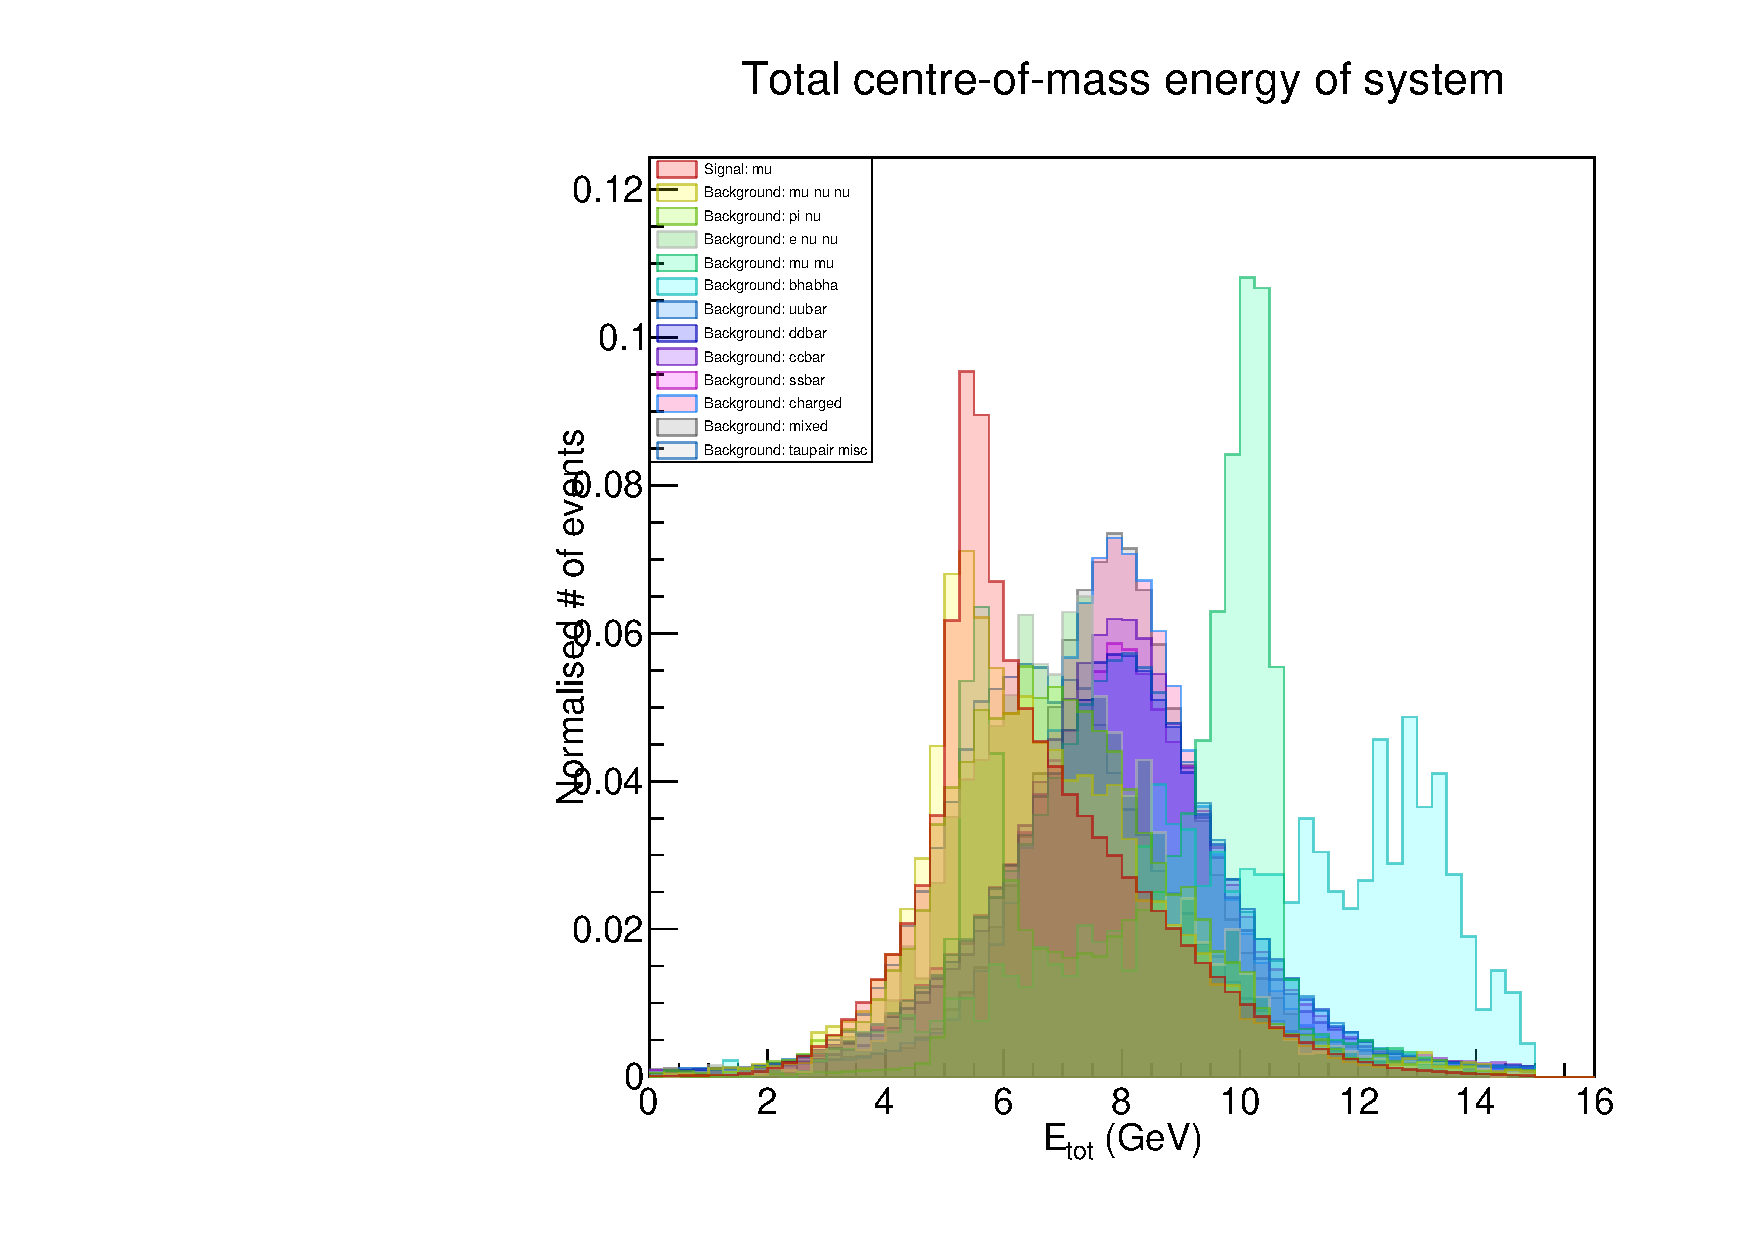
\includegraphics[width=\linewidth]{images/stack/stack_cut6_totalCM_E.pdf}
  \captionof{figure}{A figure}
  \label{fig:test1}
\end{minipage}%
\begin{minipage}{.5\textwidth}
  \centering
  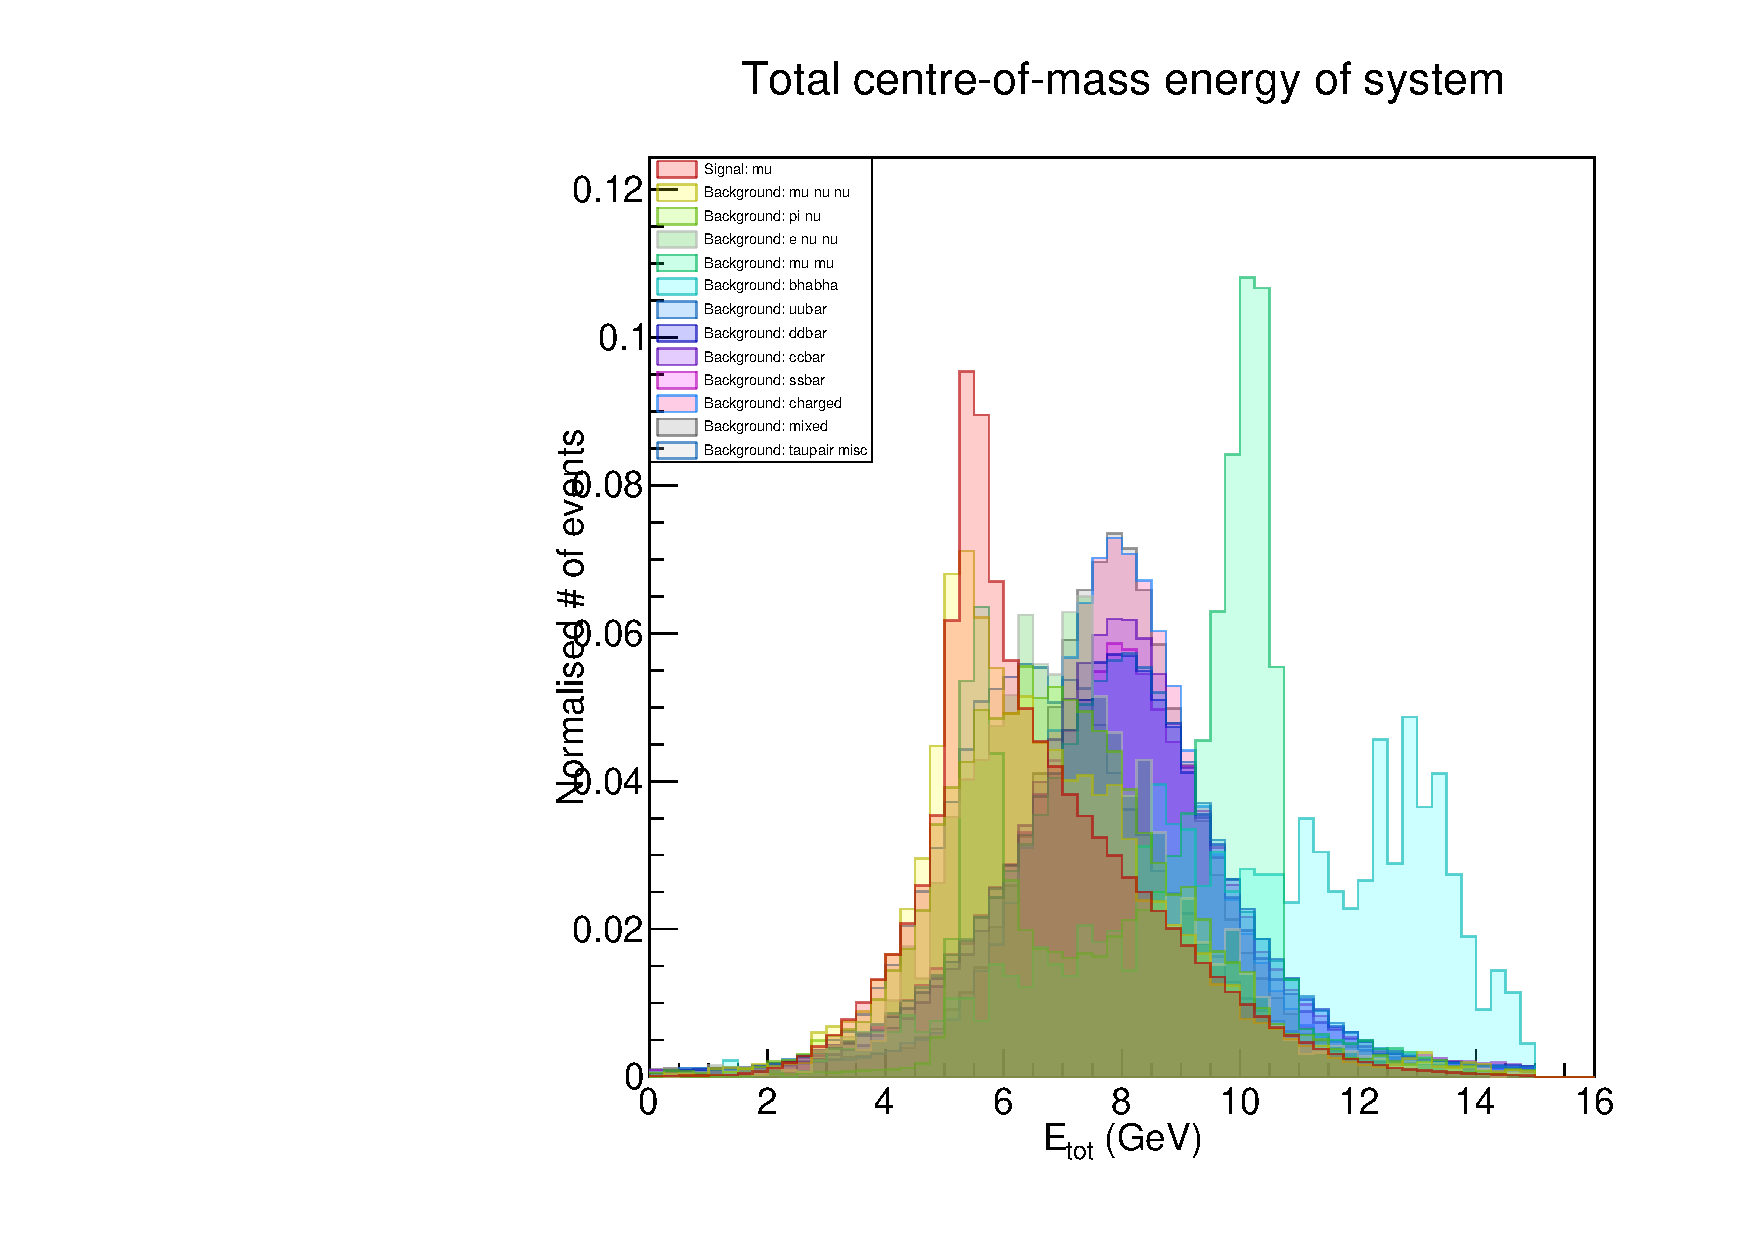
\includegraphics[width=\linewidth]{images/stack/stack_cut6_totalCM_E.pdf}
  \captionof{figure}{Another figure}
  \label{fig:test2}
\end{minipage}
\end{figure}

\subsubsection{Electron mode}

\begin{figure}[h]
\centering
\begin{minipage}{.5\textwidth}
  \centering
  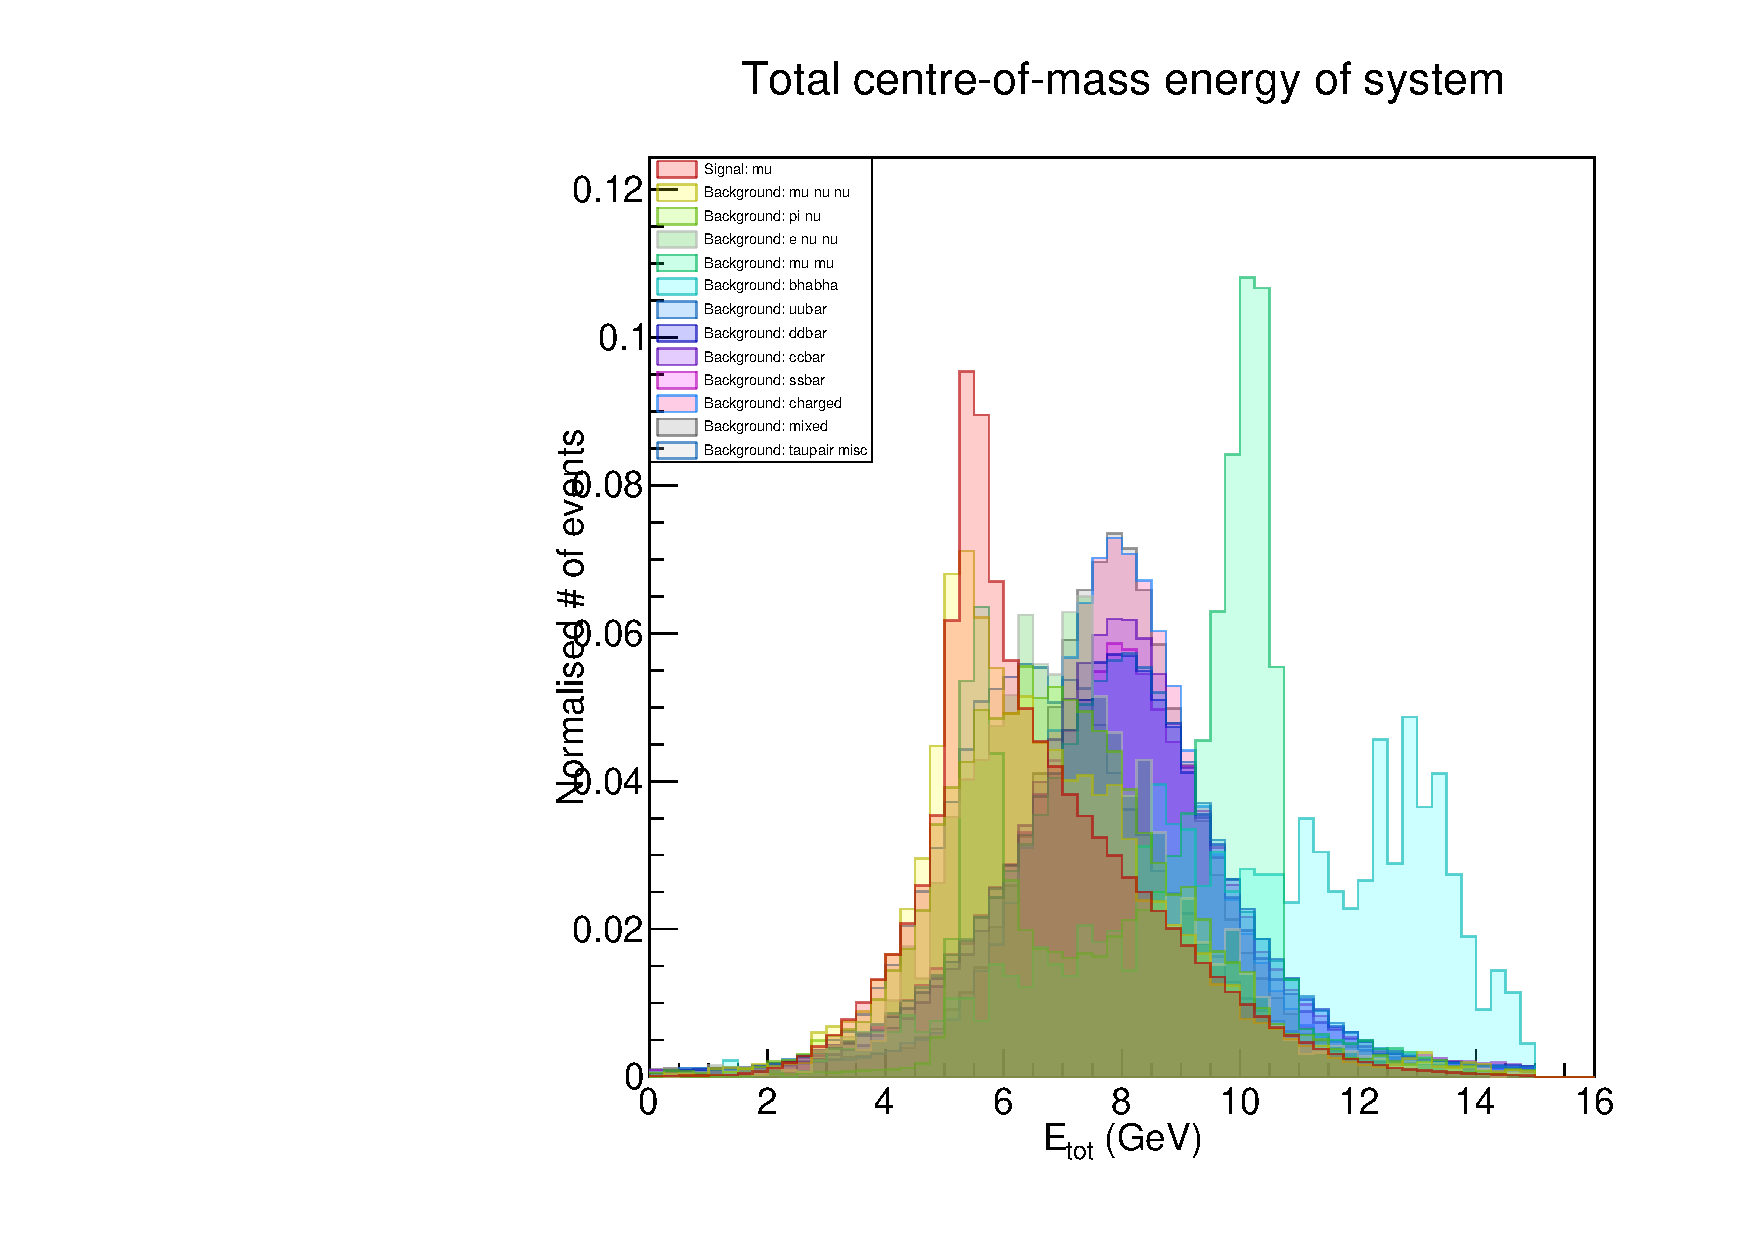
\includegraphics[width=\linewidth]{images/stack/stack_cut6_totalCM_E.pdf}
  \captionof{figure}{A figure}
  \label{fig:test1}
\end{minipage}%
\begin{minipage}{.5\textwidth}
  \centering
  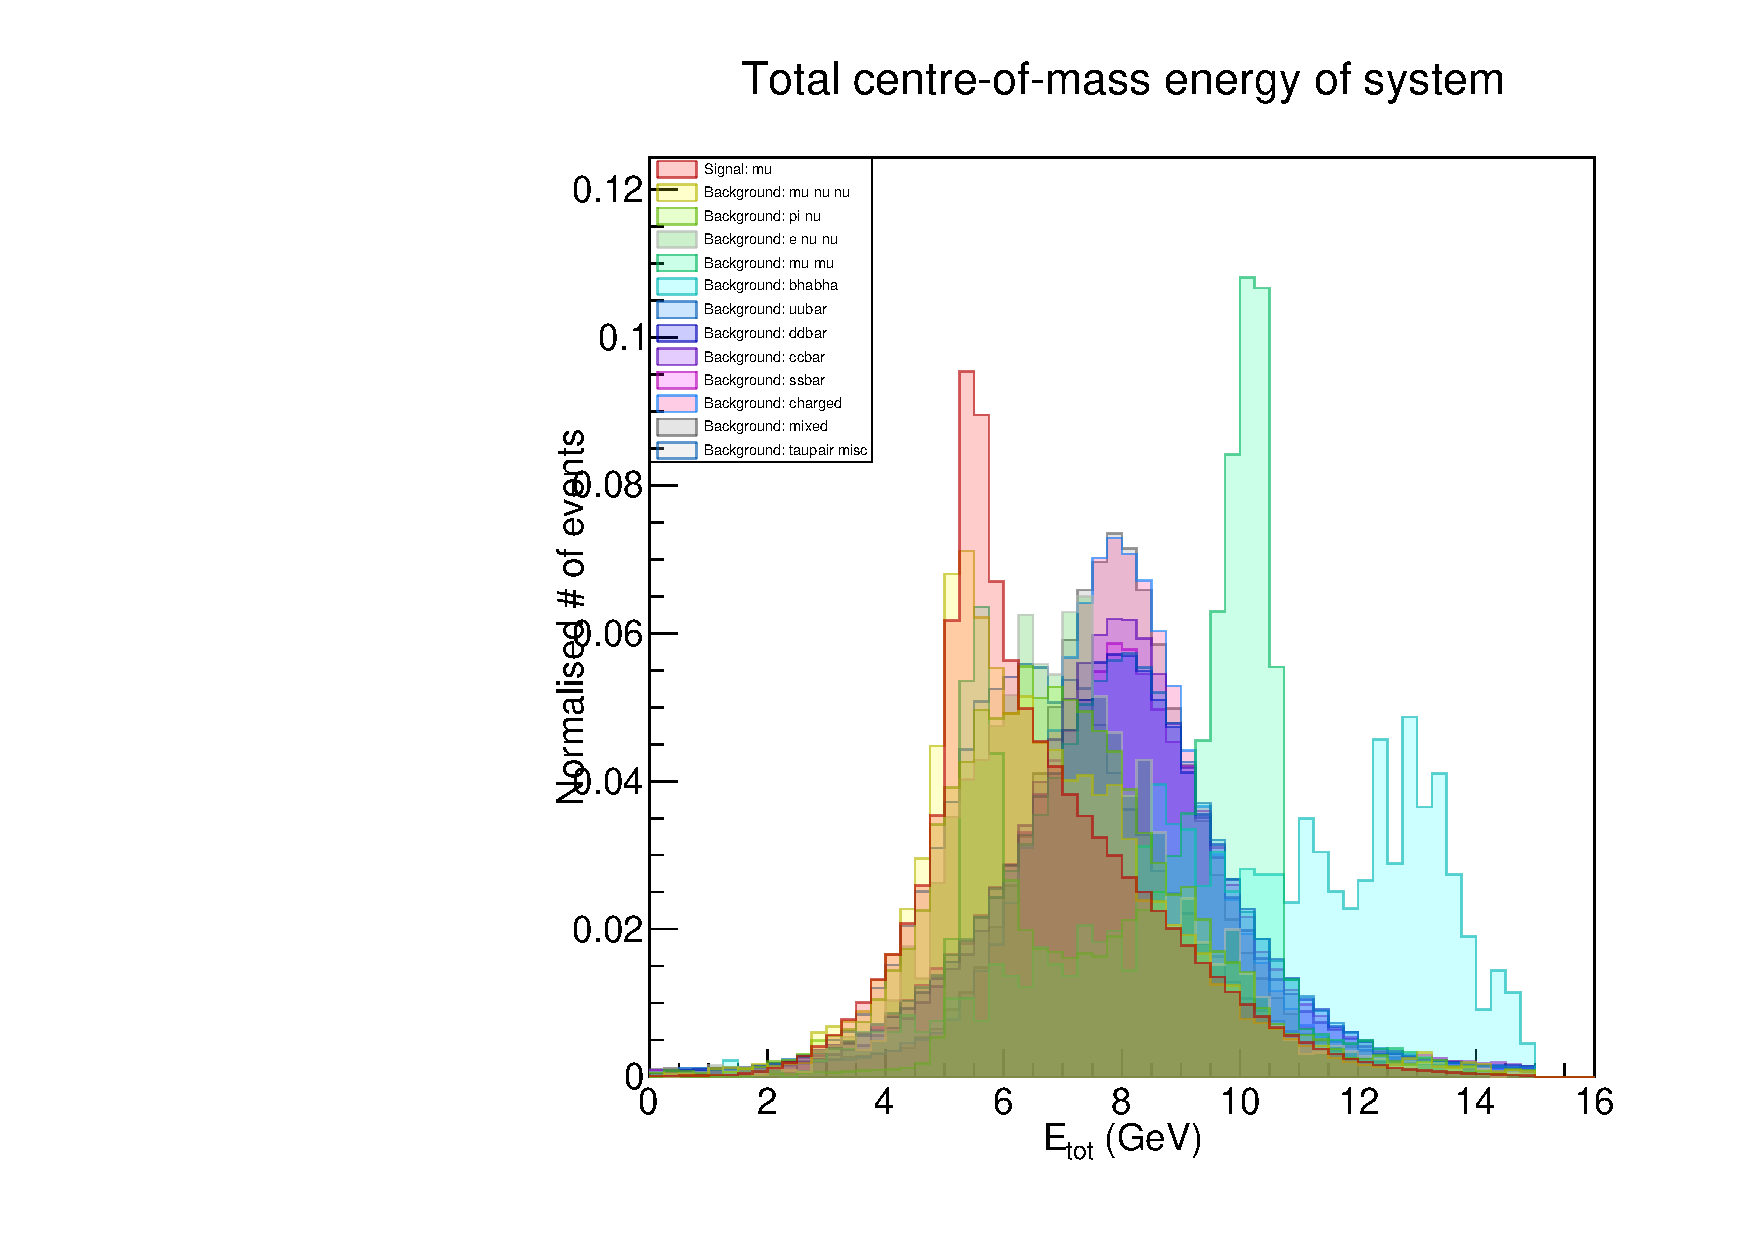
\includegraphics[width=\linewidth]{images/stack/stack_cut6_totalCM_E.pdf}
  \captionof{figure}{Another figure}
  \label{fig:test2}
\end{minipage}
\end{figure}


\subsection{Backgrounds}

\subsubsection{Tau-pair processes}

\begin{figure}[h]
\centering
\begin{minipage}{.5\textwidth}
  \centering
  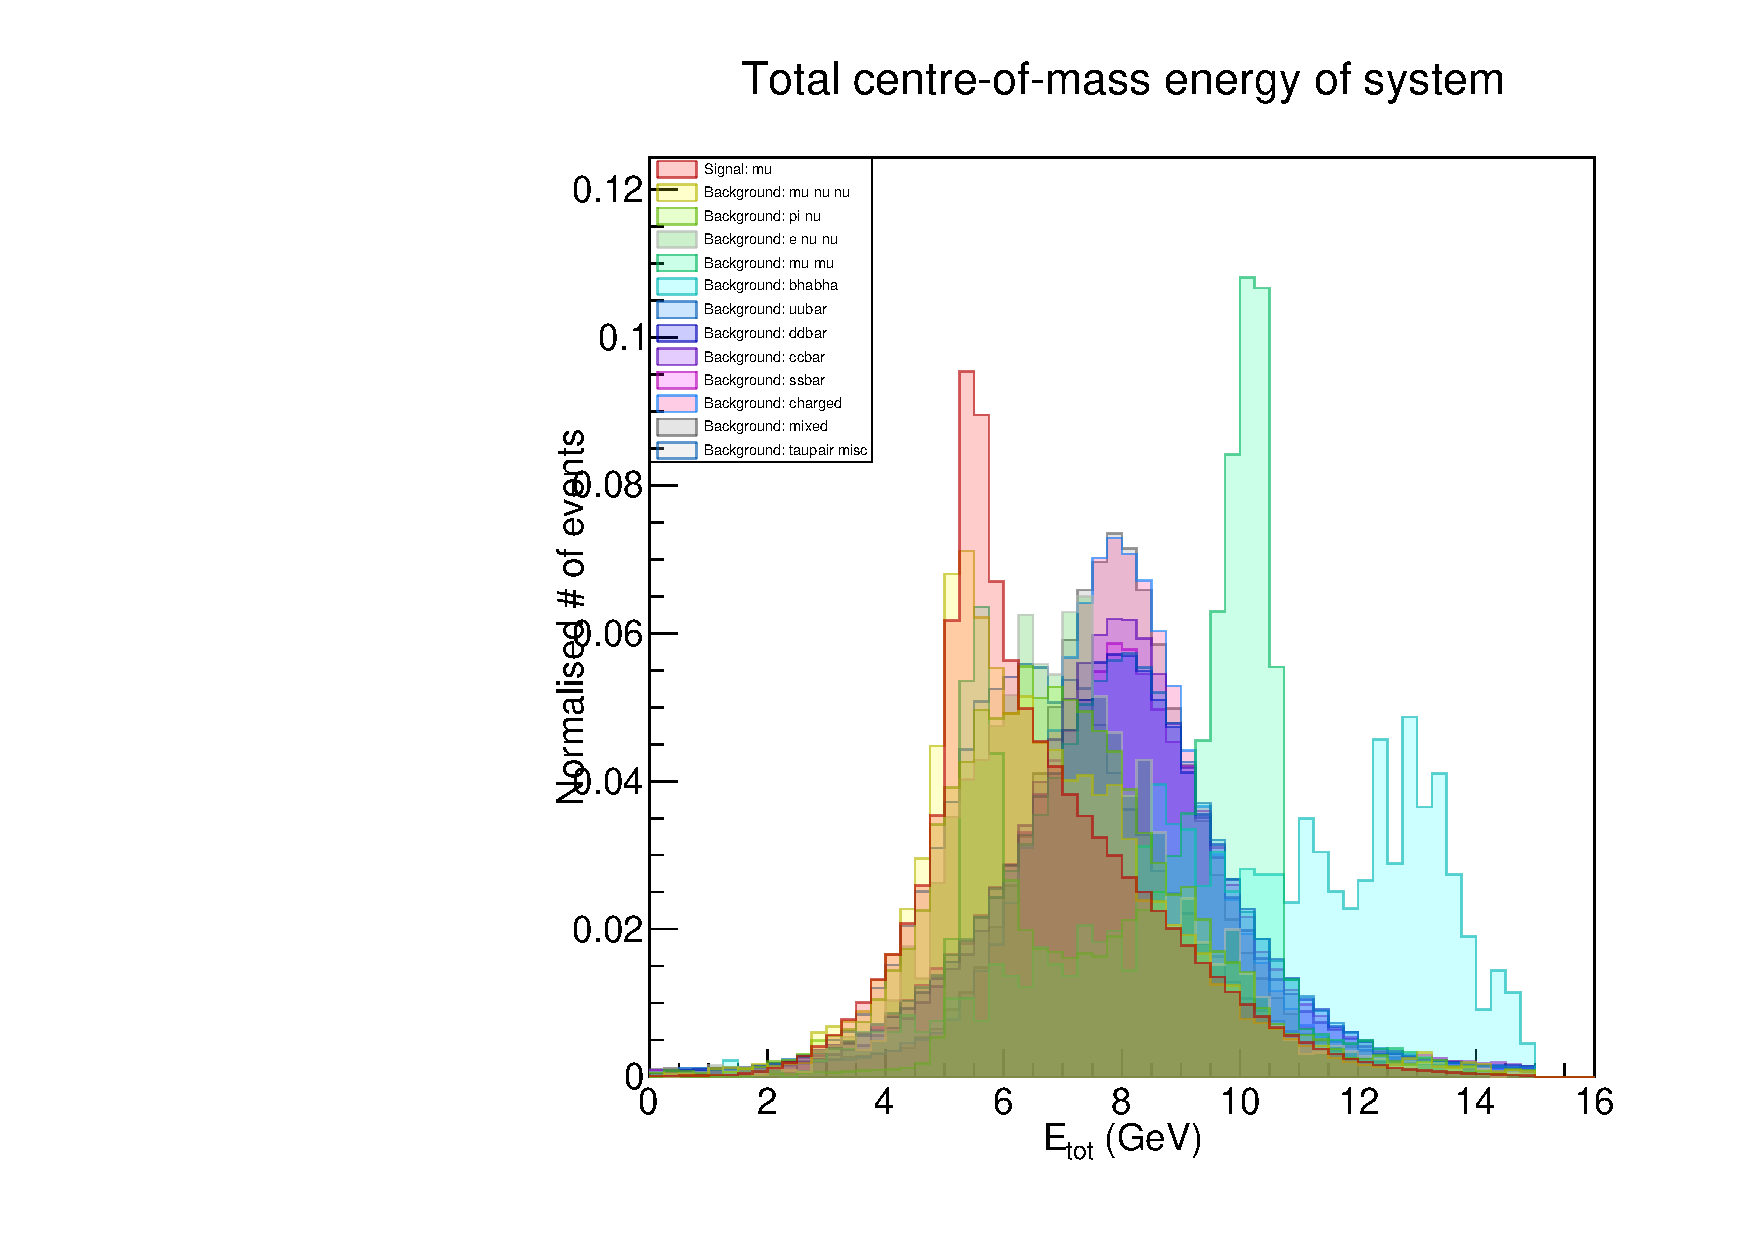
\includegraphics[width=\linewidth]{images/stack/stack_cut6_totalCM_E.pdf}
  \captionof{figure}{A figure}
  \label{fig:test1}
\end{minipage}%
\begin{minipage}{.5\textwidth}
  \centering
  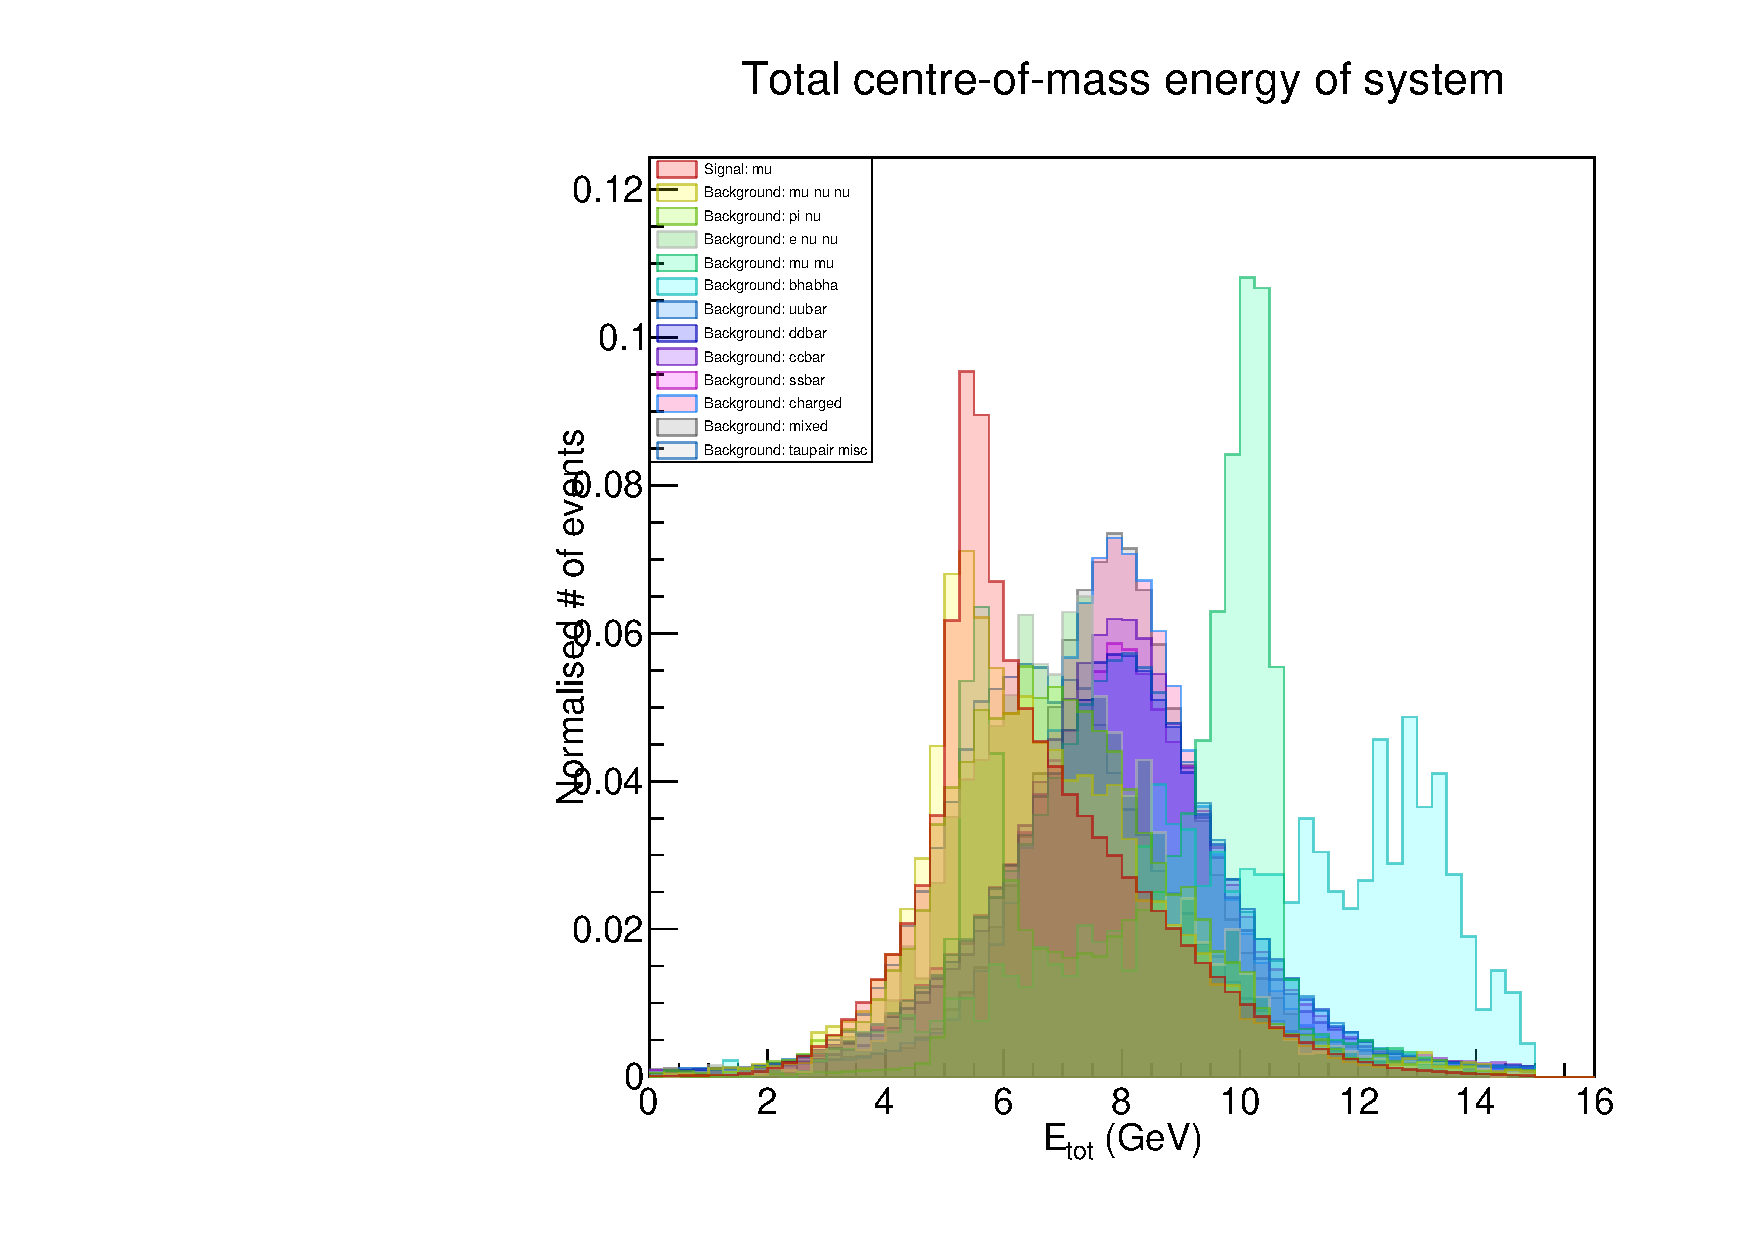
\includegraphics[width=\linewidth]{images/stack/stack_cut6_totalCM_E.pdf}
  \captionof{figure}{Another figure}
  \label{fig:test2}
\end{minipage}
\end{figure}



\subsubsection{Mu-pair processes}

\begin{figure}[h]
\centering
\begin{minipage}{.5\textwidth}
  \centering
  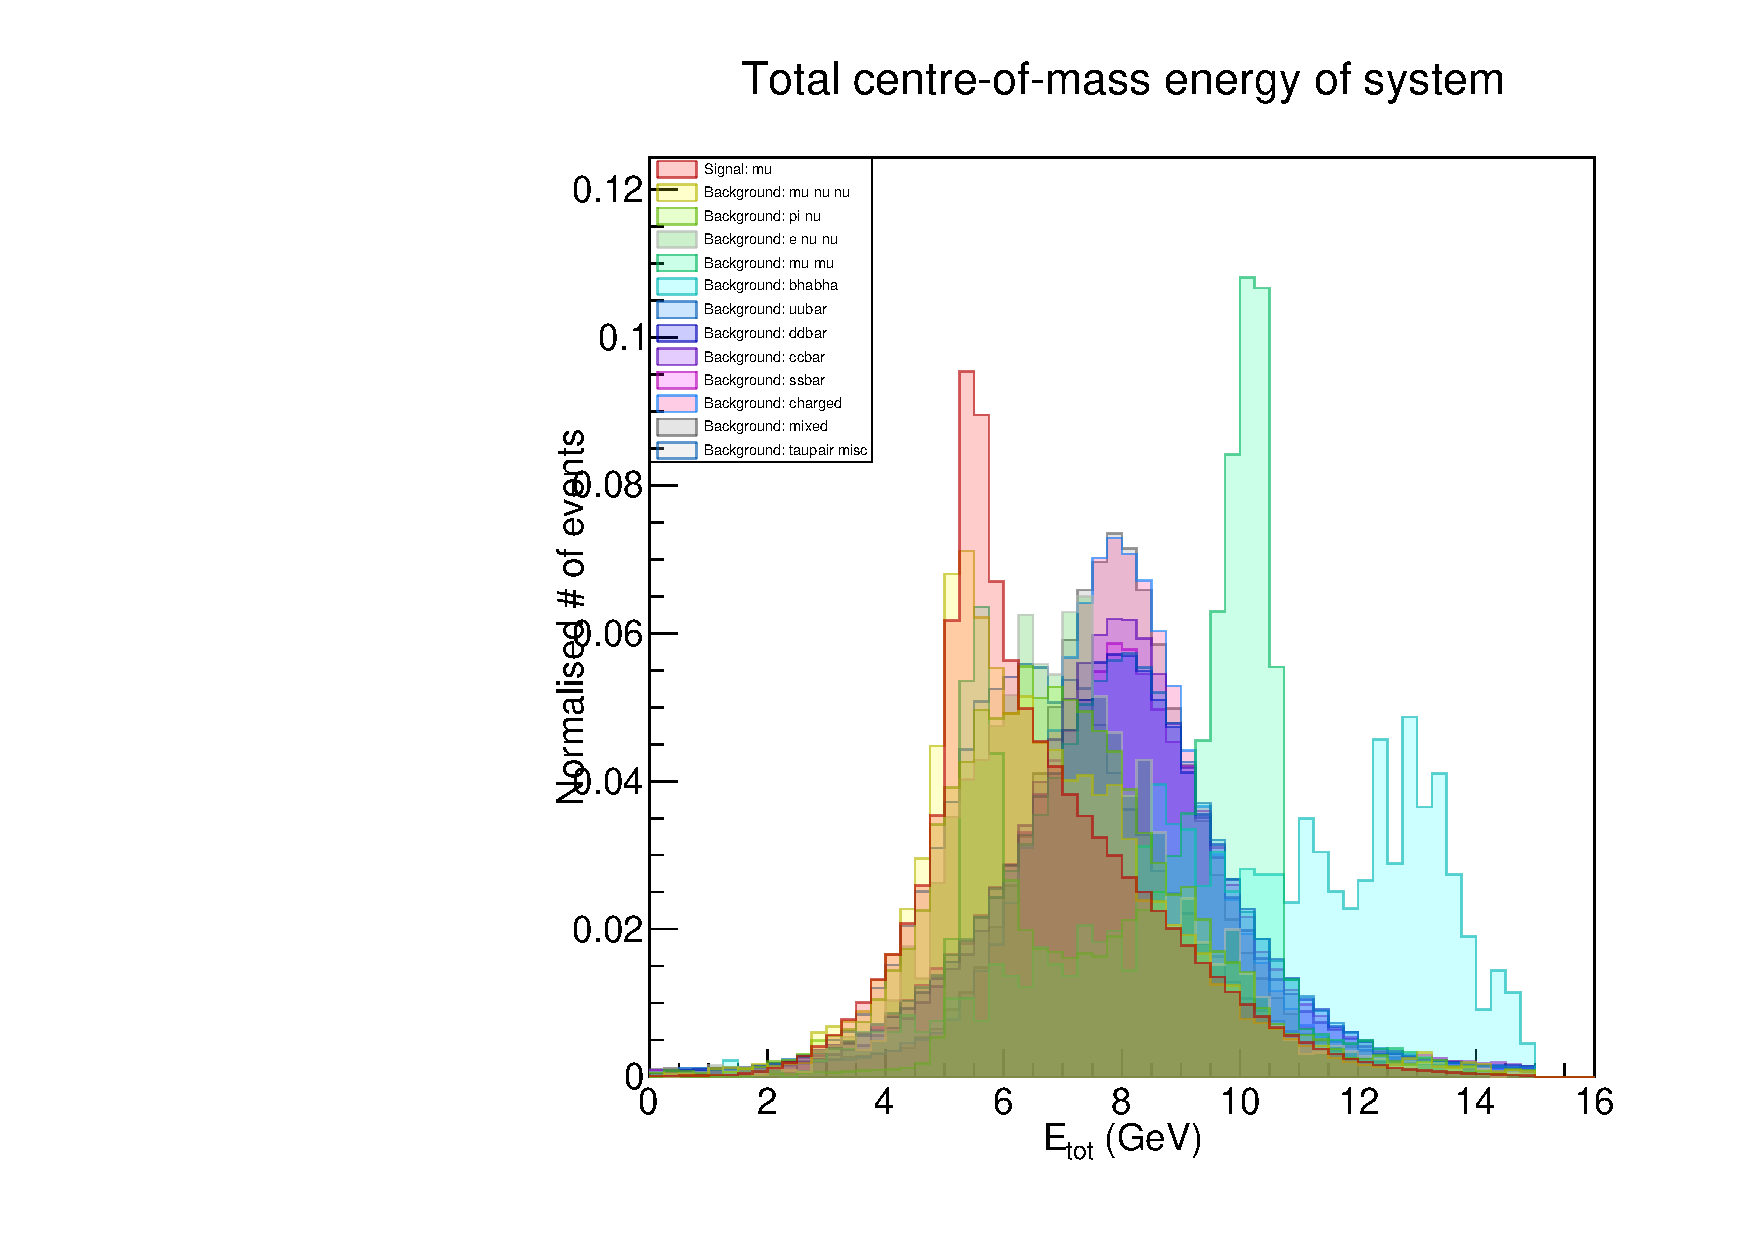
\includegraphics[width=\linewidth]{images/stack/stack_cut6_totalCM_E.pdf}
  \captionof{figure}{A figure}
  \label{fig:test1}
\end{minipage}%
\begin{minipage}{.5\textwidth}
  \centering
  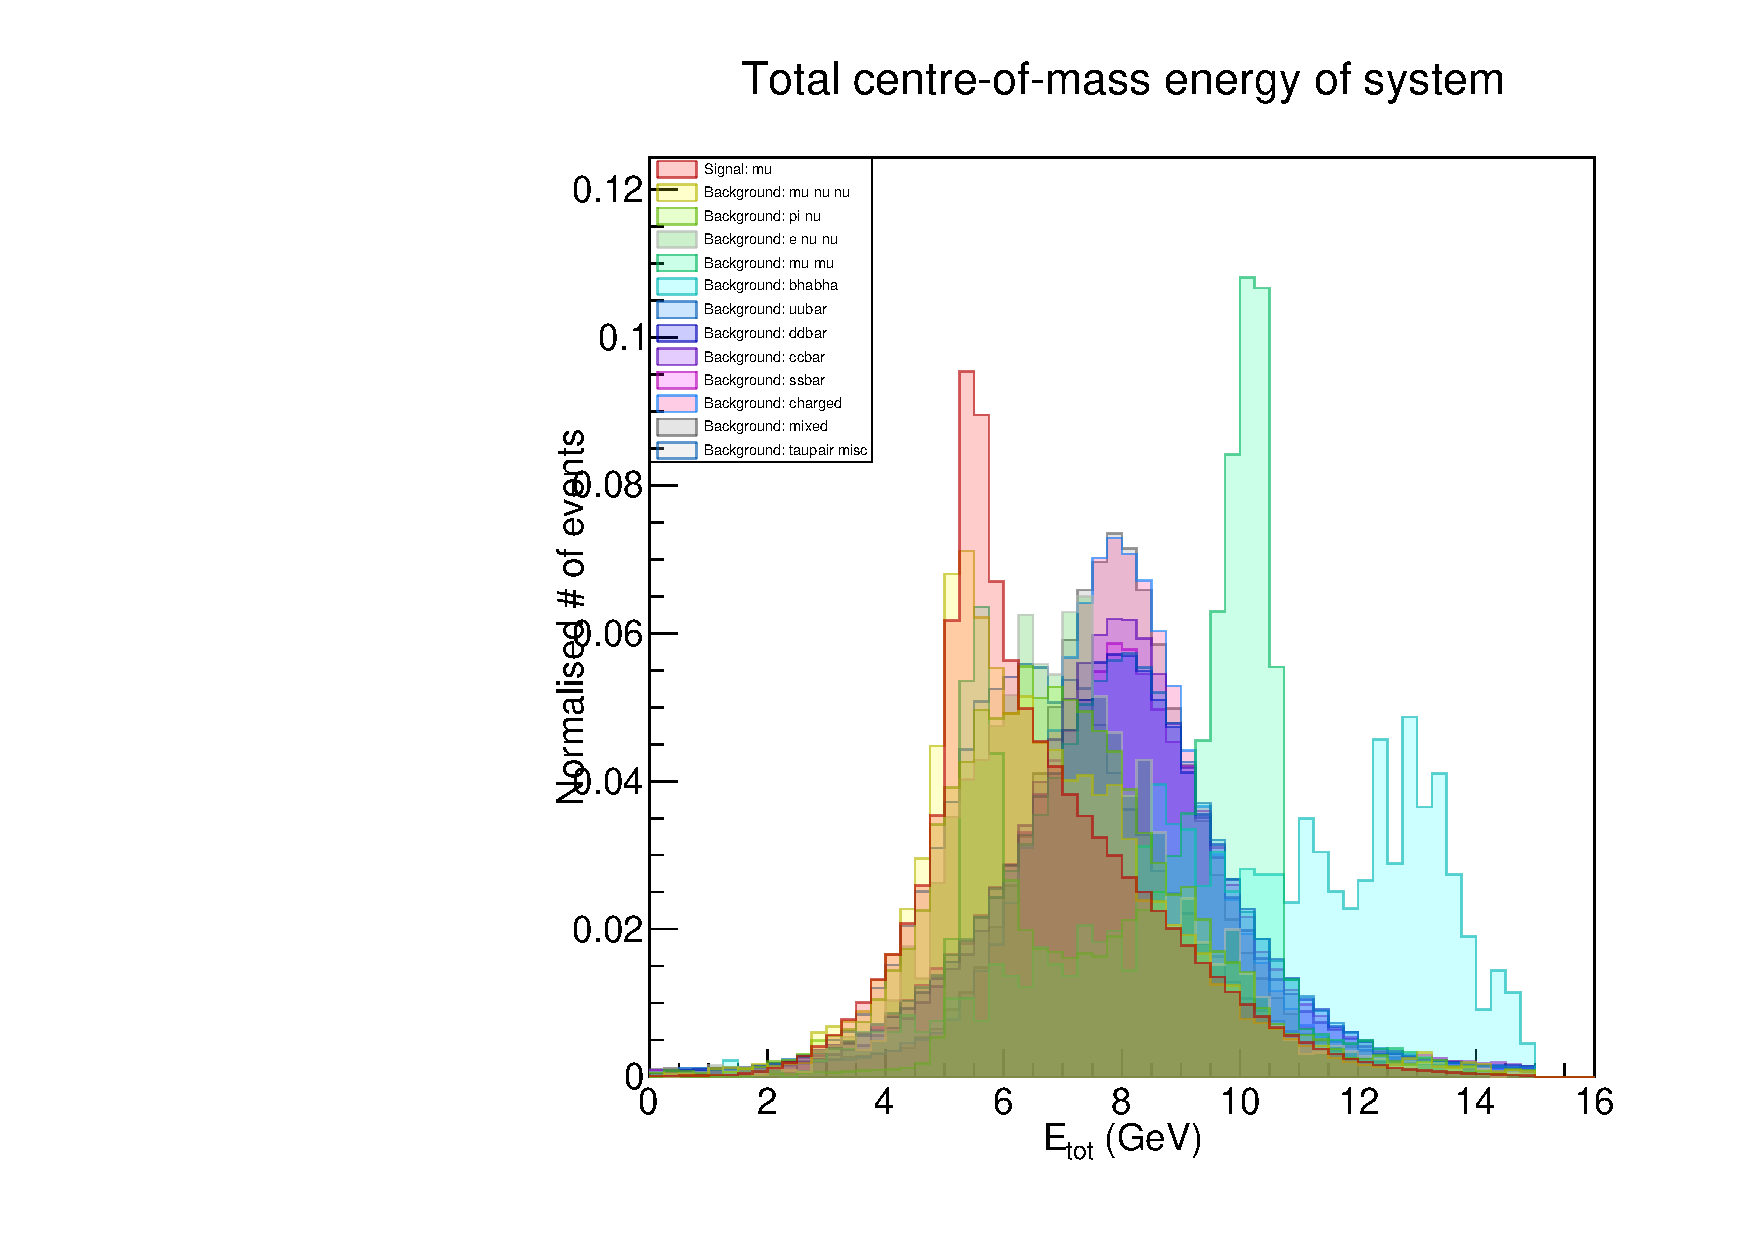
\includegraphics[width=\linewidth]{images/stack/stack_cut6_totalCM_E.pdf}
  \captionof{figure}{Another figure}
  \label{fig:test2}
\end{minipage}
\end{figure}

\subsubsection{Bhabha}

\begin{figure}[h]
\centering
\begin{minipage}{.5\textwidth}
  \centering
  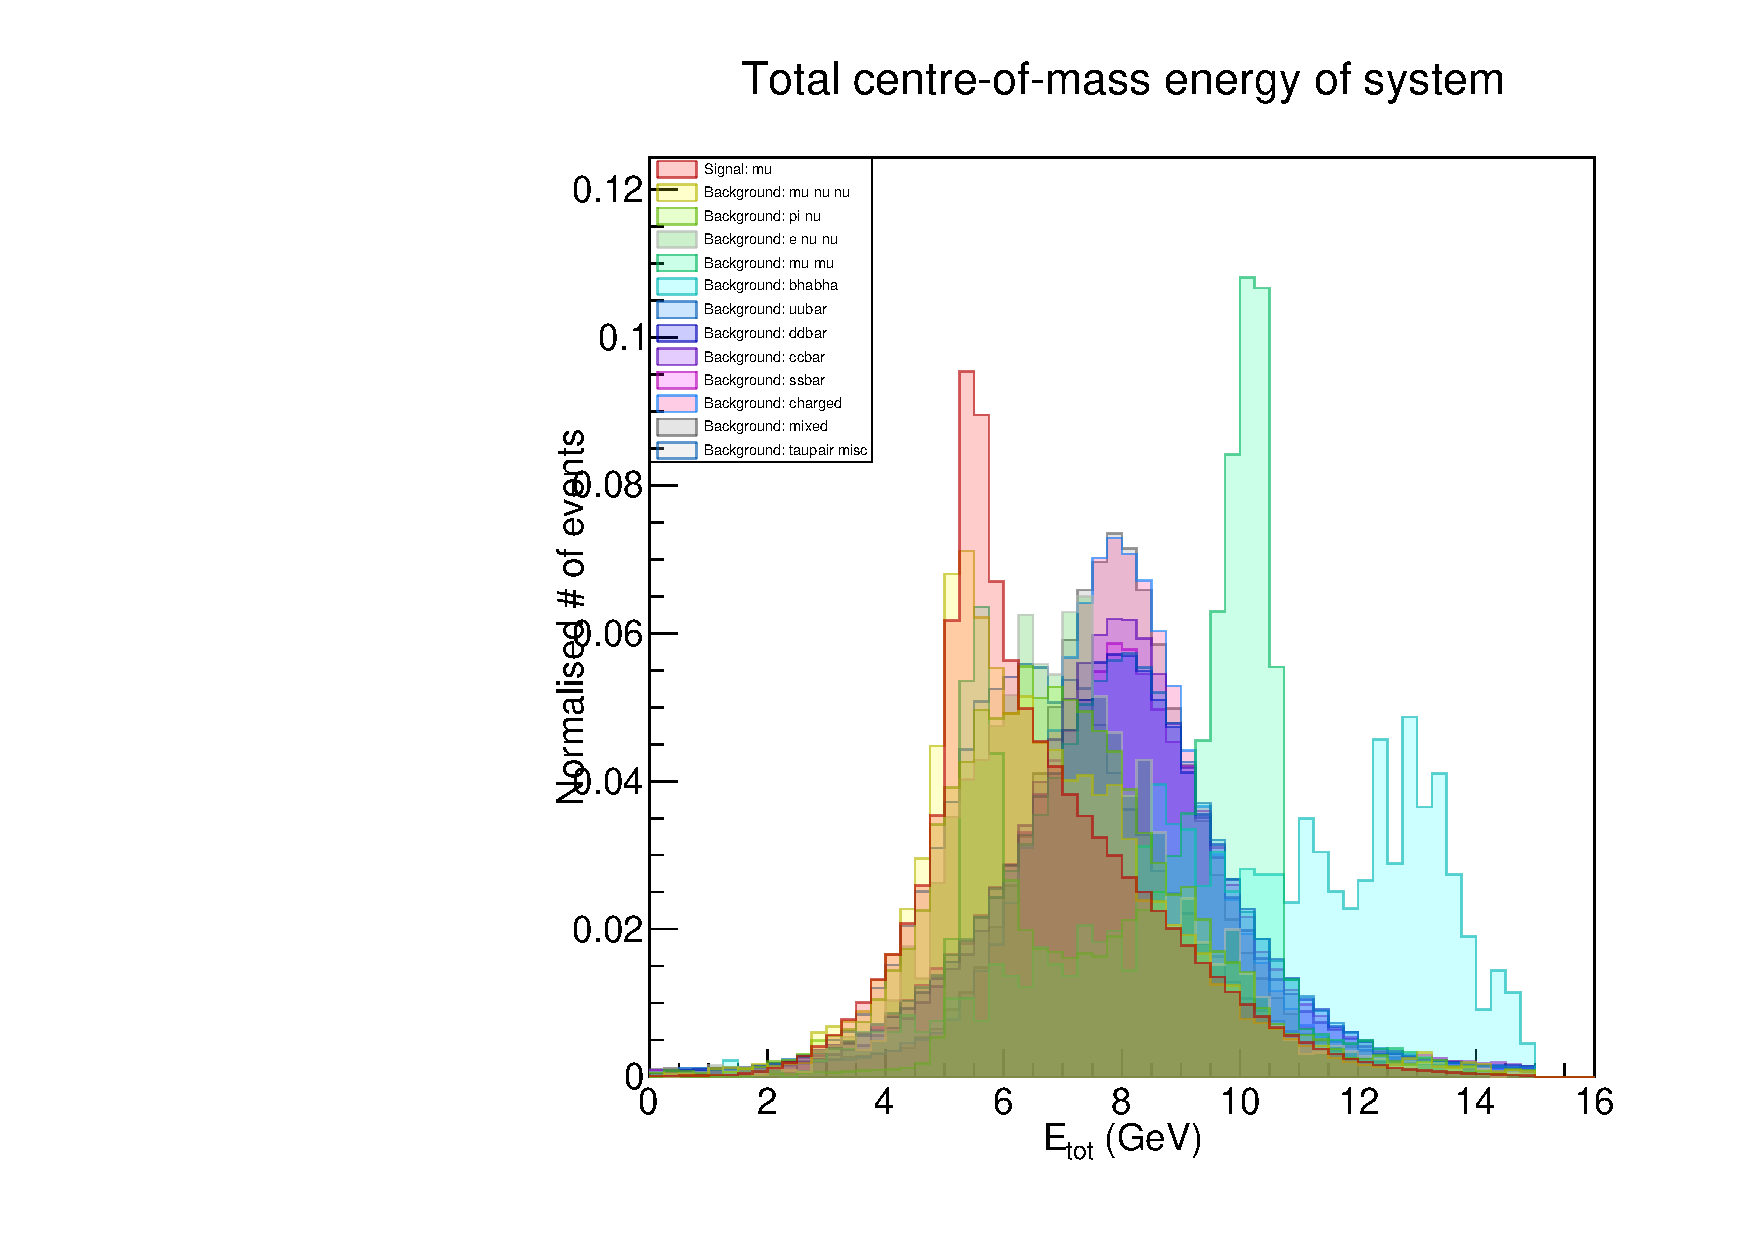
\includegraphics[width=\linewidth]{images/stack/stack_cut6_totalCM_E.pdf}
  \captionof{figure}{A figure}
  \label{fig:test1}
\end{minipage}%
\begin{minipage}{.5\textwidth}
  \centering
  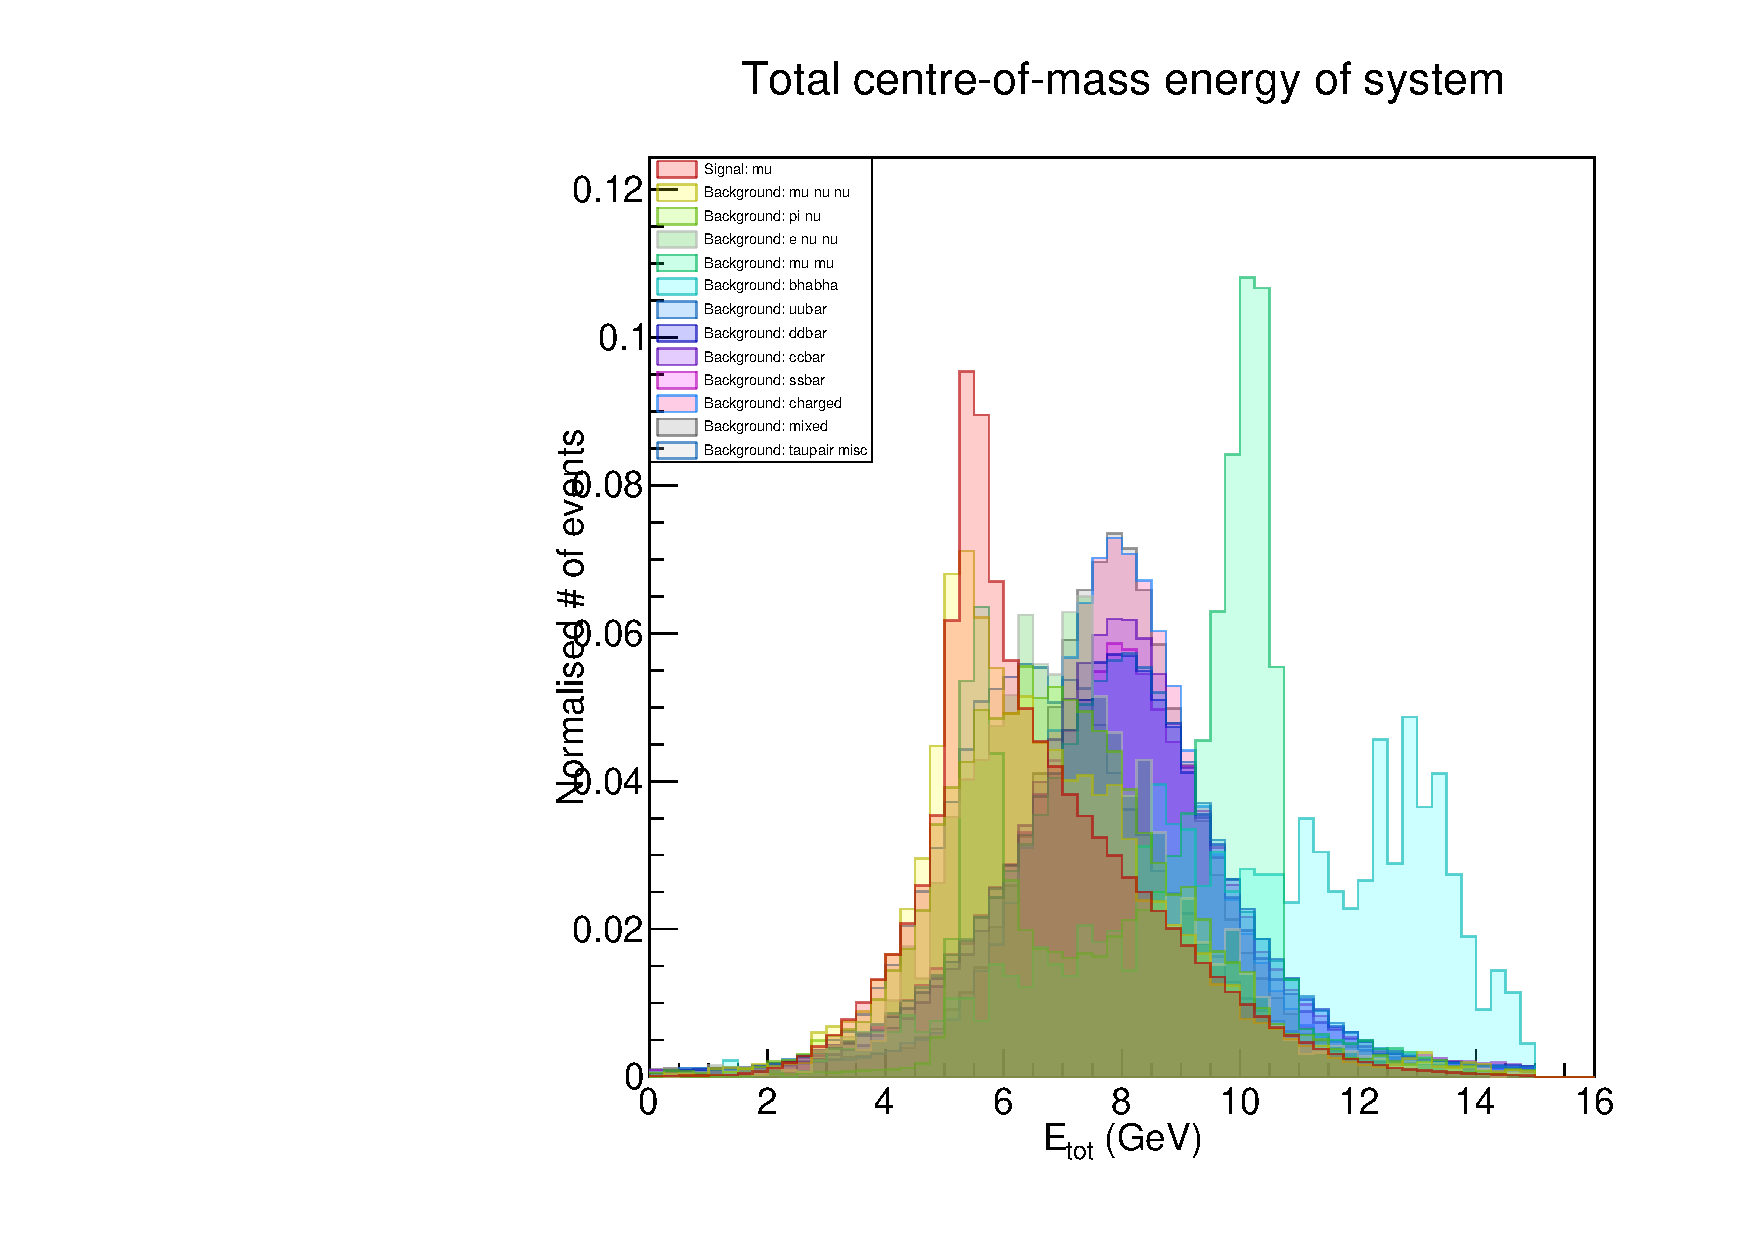
\includegraphics[width=\linewidth]{images/stack/stack_cut6_totalCM_E.pdf}
  \captionof{figure}{Another figure}
  \label{fig:test2}
\end{minipage}
\end{figure}

\subsubsection{Continuum and $B\bar{B}$}

    \begin{figure*}
        \centering
        \begin{subfigure}[b]{0.475\textwidth}
            \centering
            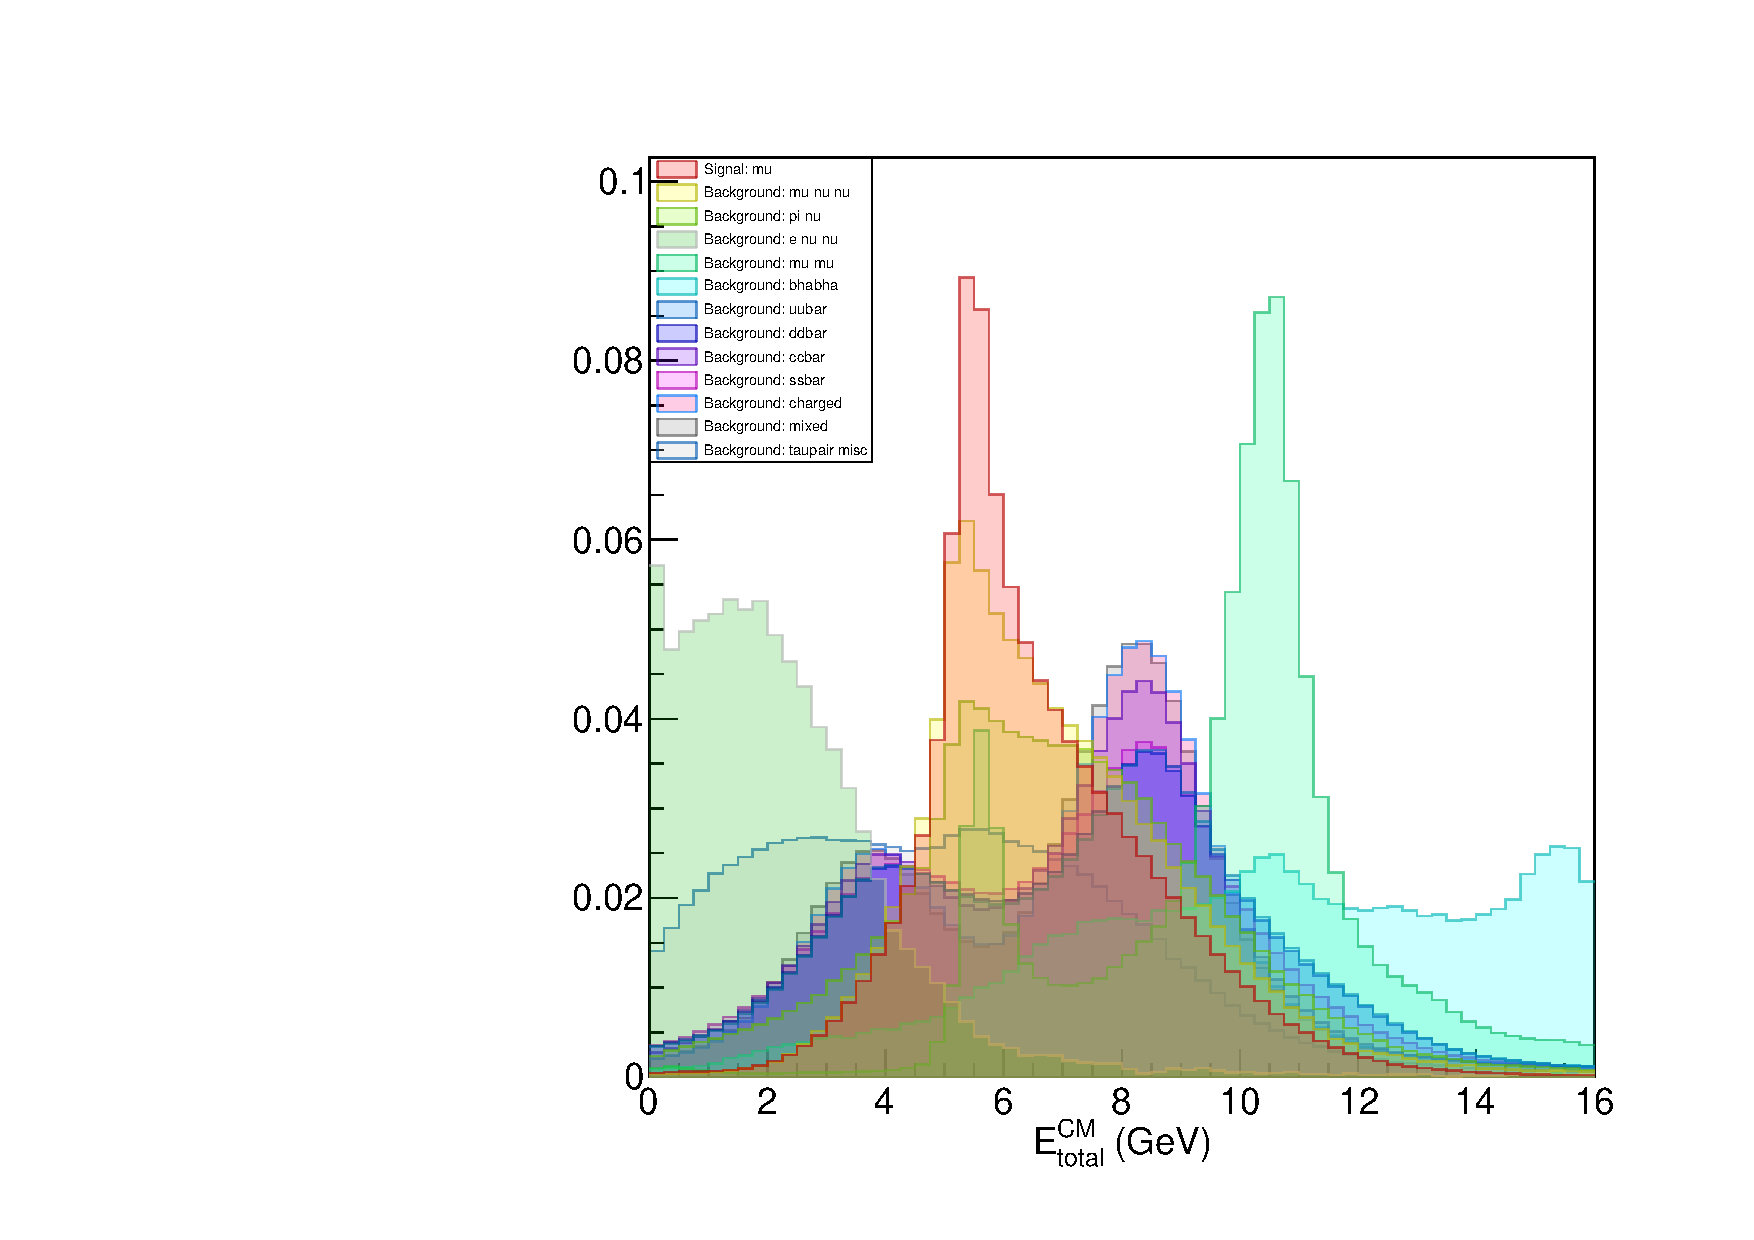
\includegraphics[width=\textwidth]{images/test.pdf}
            \caption[Network2]%
            {{\small Network 1}}    
            \label{fig:mean and std of net14}
        \end{subfigure}
        \hfill
        \begin{subfigure}[b]{0.475\textwidth}  
            \centering 
            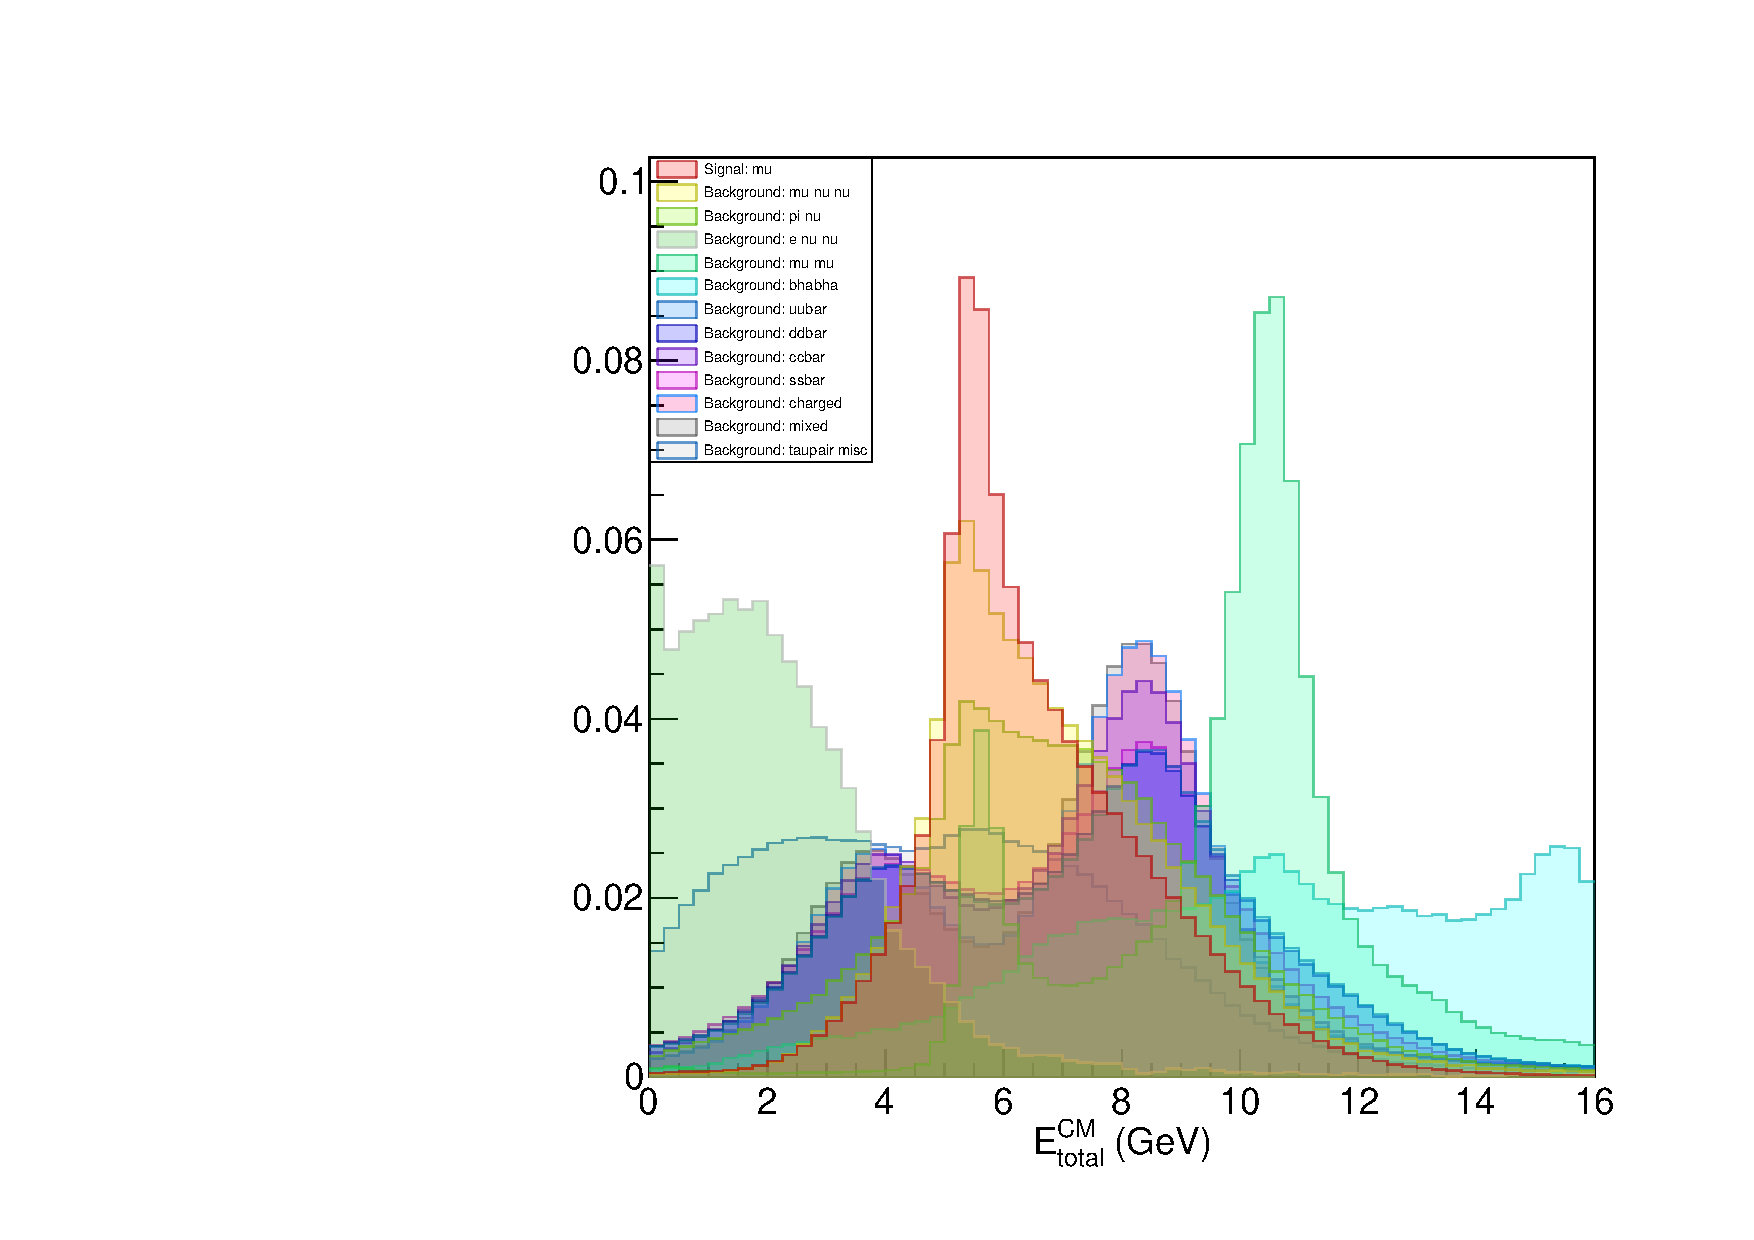
\includegraphics[width=\textwidth]{images/test.pdf}
            \caption[]%
            {{\small Network 2}}    
            \label{fig:mean and std of net24}
        \end{subfigure}
        \vskip\baselineskip
        \begin{subfigure}[b]{0.475\textwidth}   
            \centering 
            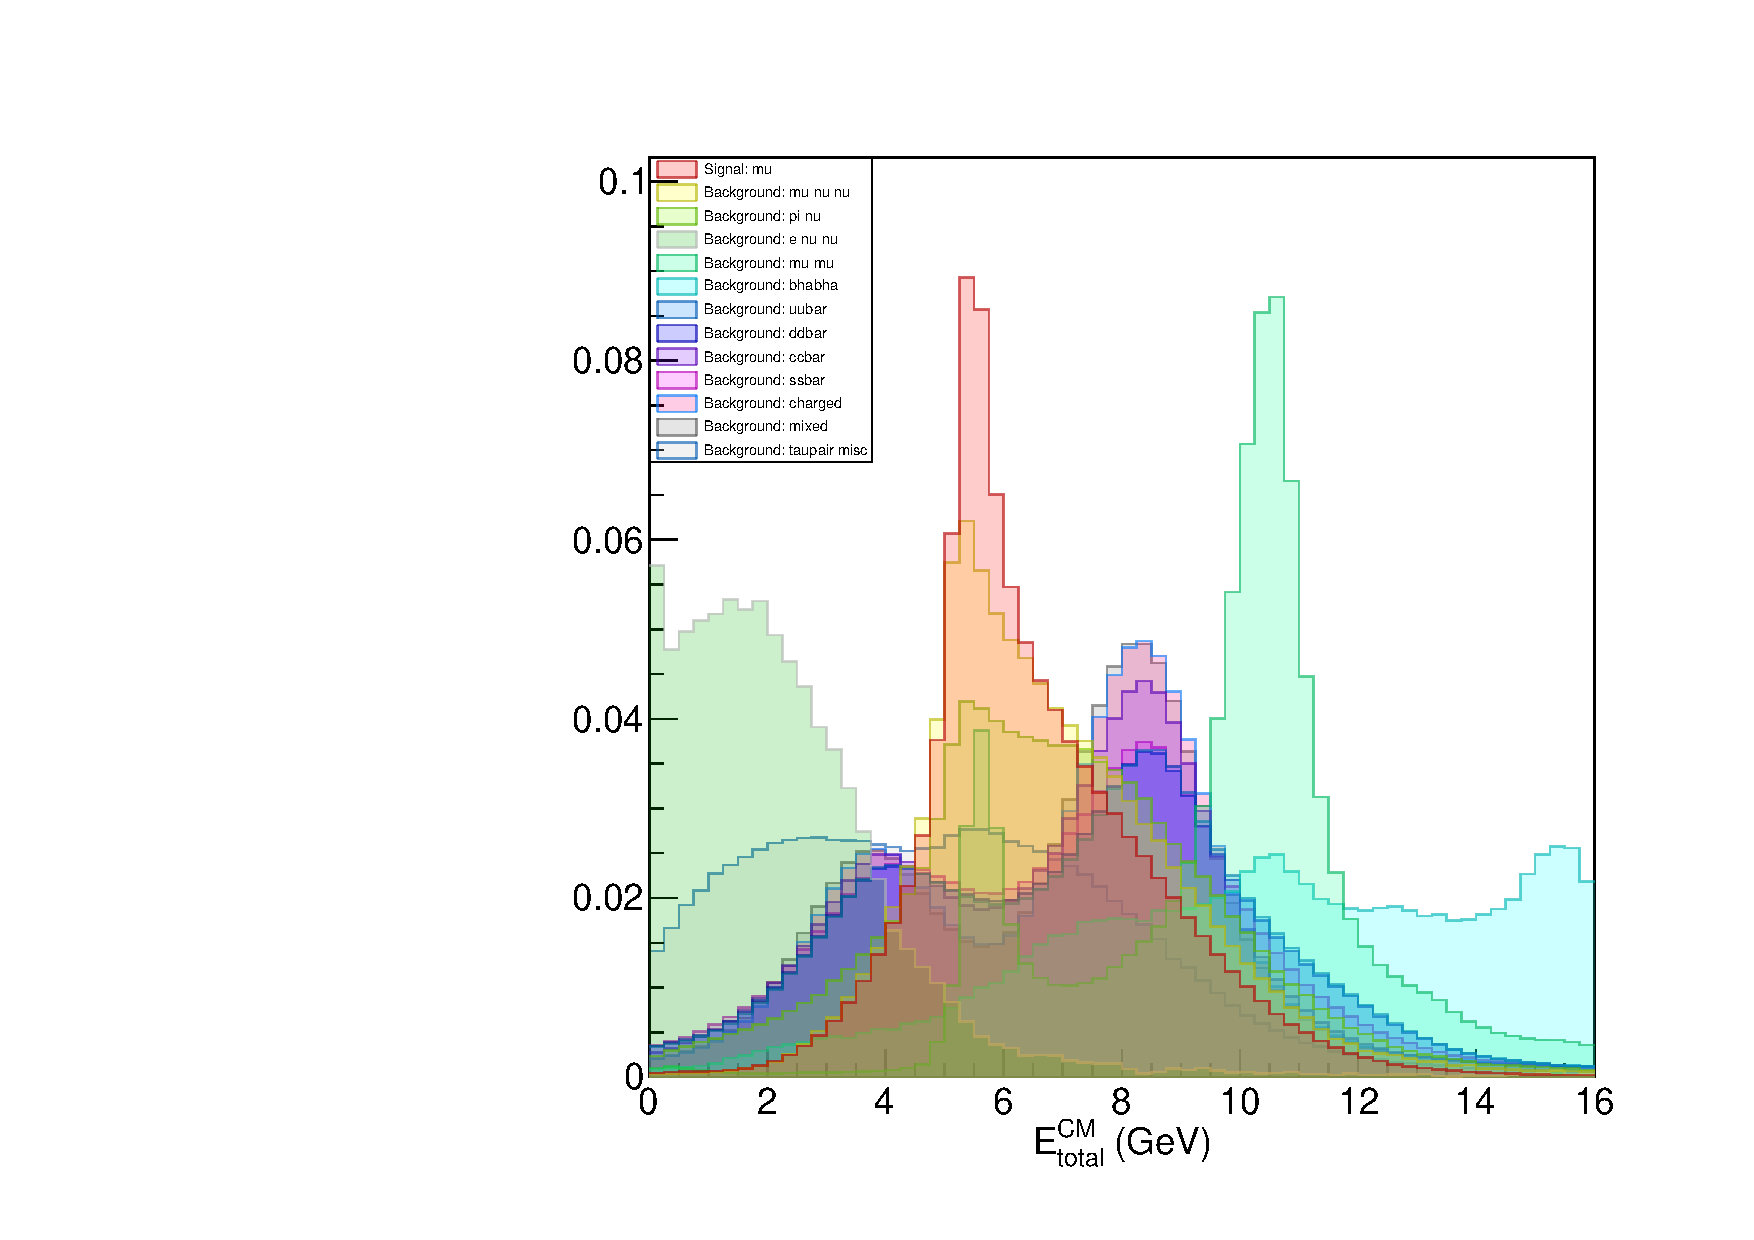
\includegraphics[width=\textwidth]{images/test.pdf}
            \caption[]%
            {{\small Network 3}}    
            \label{fig:mean and std of net34}
        \end{subfigure}
        \quad
        \begin{subfigure}[b]{0.475\textwidth}   
            \centering 
            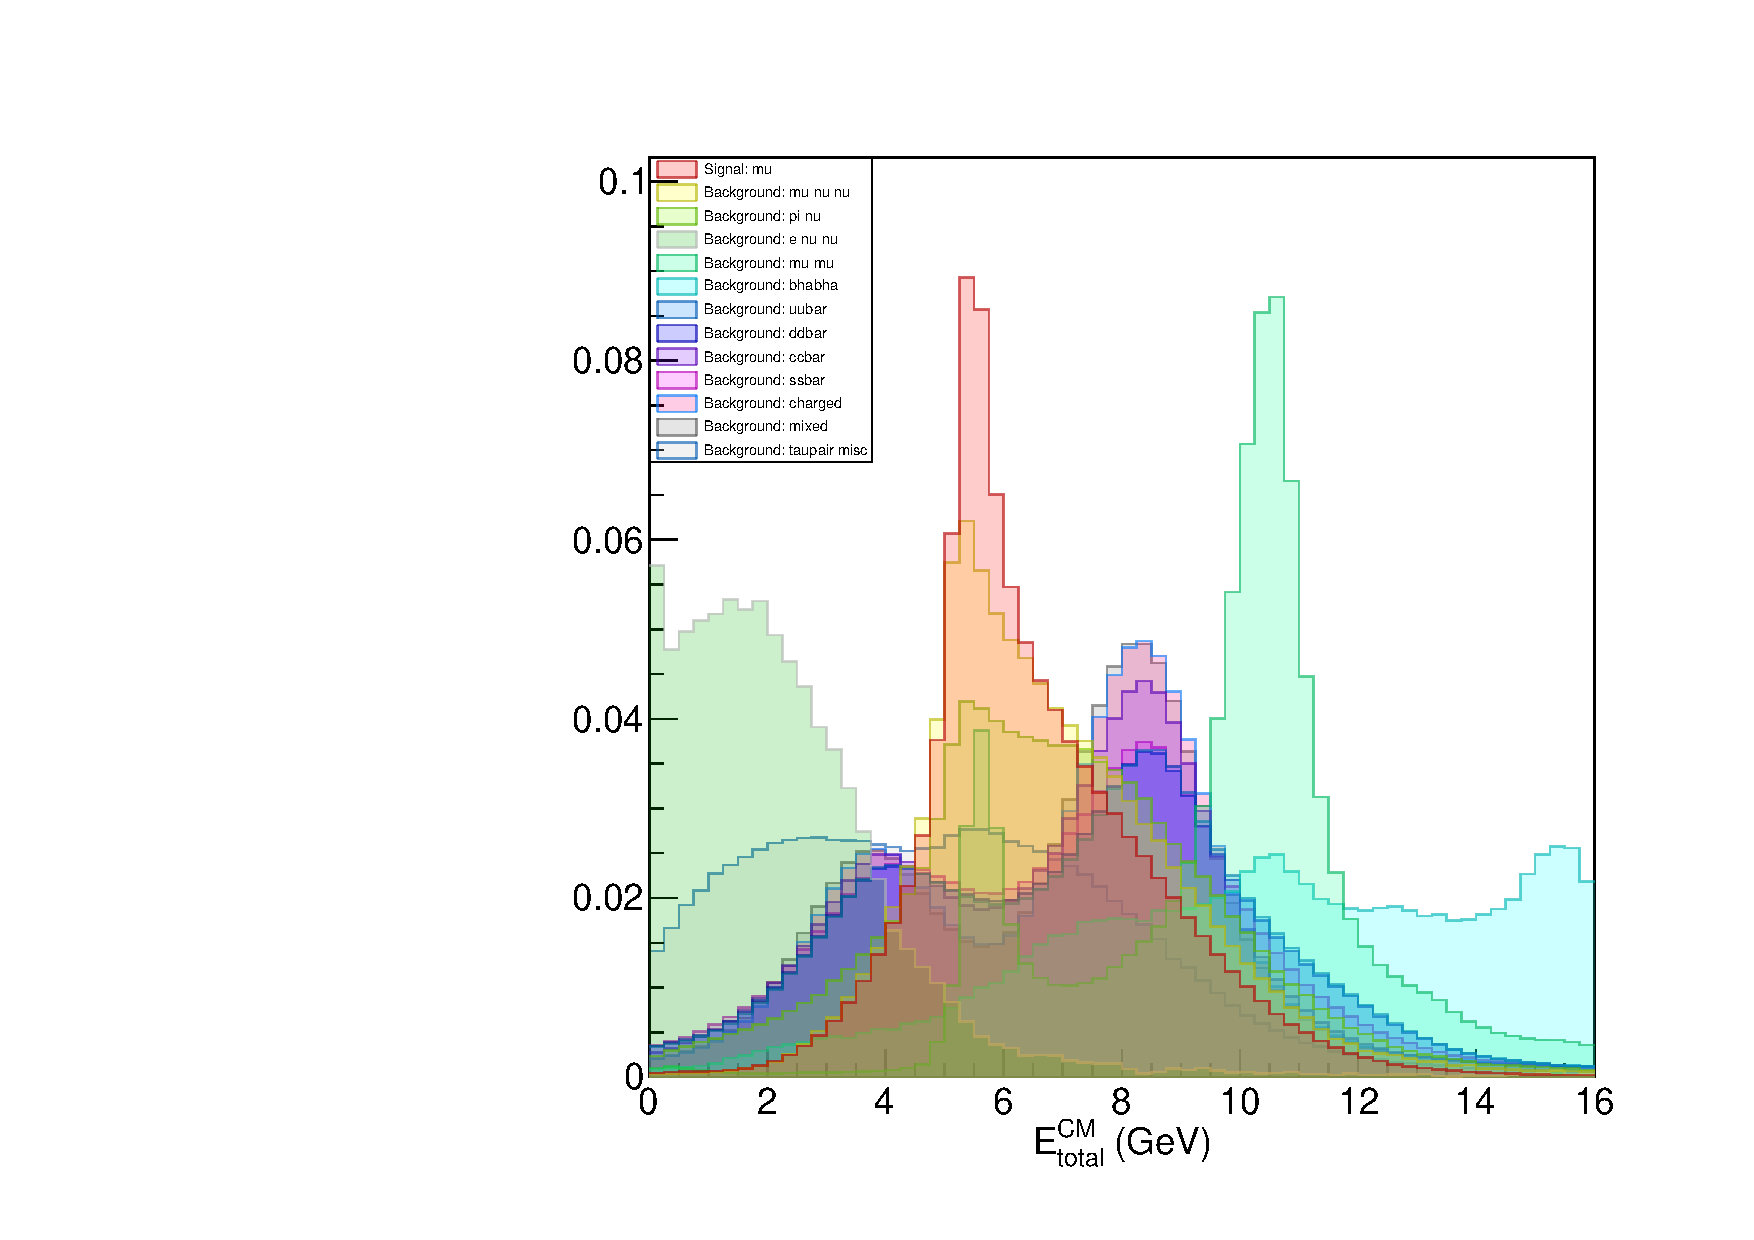
\includegraphics[width=\textwidth]{images/test.pdf}
            \caption[]%
            {{\small Network 4}}    
            \label{fig:mean and std of net44}
        \end{subfigure}
        \caption[ The average and standard deviation of critical parameters ]
        {\small The average and standard deviation of critical parameters: Region R4} 
        \label{fig:mean and std of nets}
    \end{figure*}


\pagebreak

%-------------------------------------------------------------------

\section{Preselection}

Following reconstruction, preselection criteria were applied to the reconstructed ROOT files. Preselection criteria are distinct from selection criteria in that they remove a minimal amount of signal while removing the more obvious background components; in choosing selection criteria we seek to maximise $S/\sqrt{S+B}$, which may necessarily involve ``cutting out'' some non-neglible amount of signal.

The preselection criteria were selected by inspection of plots of various topology and energy based variables.  The final state modes $\tau\to\mu\gamma$ and $\tau\to e\gamma$ have differing profiles across a range of variables, so different preselection and selection criteria need to be optimised for each mode. 


\subsection{Muon mode}
Figures xxx - xxx below show the variables on which preselection criteria were applied, with the specific values for preselection listed in Table xxx.

\begin{figure}[h]
\centering
\begin{minipage}{.5\textwidth}
  \centering
  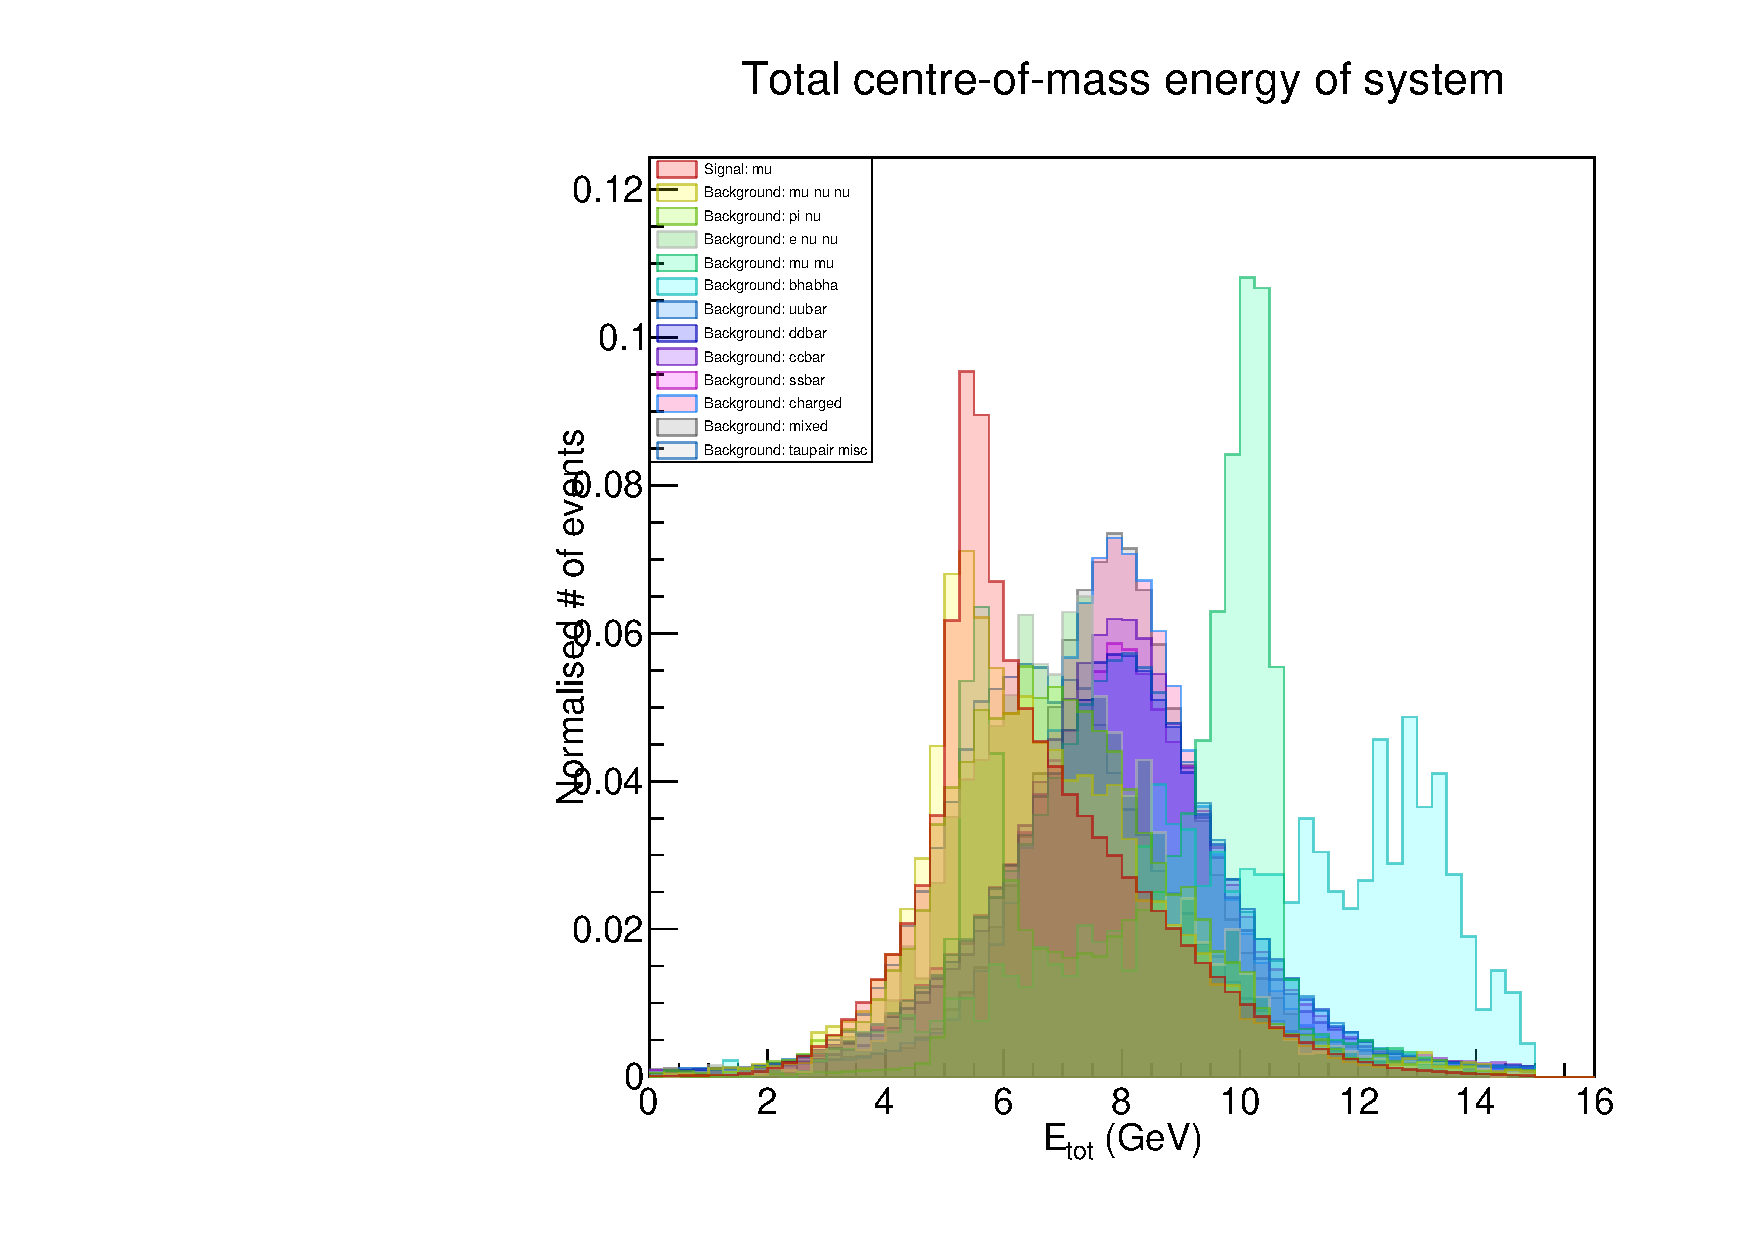
\includegraphics[width=\linewidth]{images/stack/stack_cut6_totalCM_E.pdf}
  \captionof{figure}{A figure}
  \label{fig:test1}
\end{minipage}%
\begin{minipage}{.5\textwidth}
  \centering
  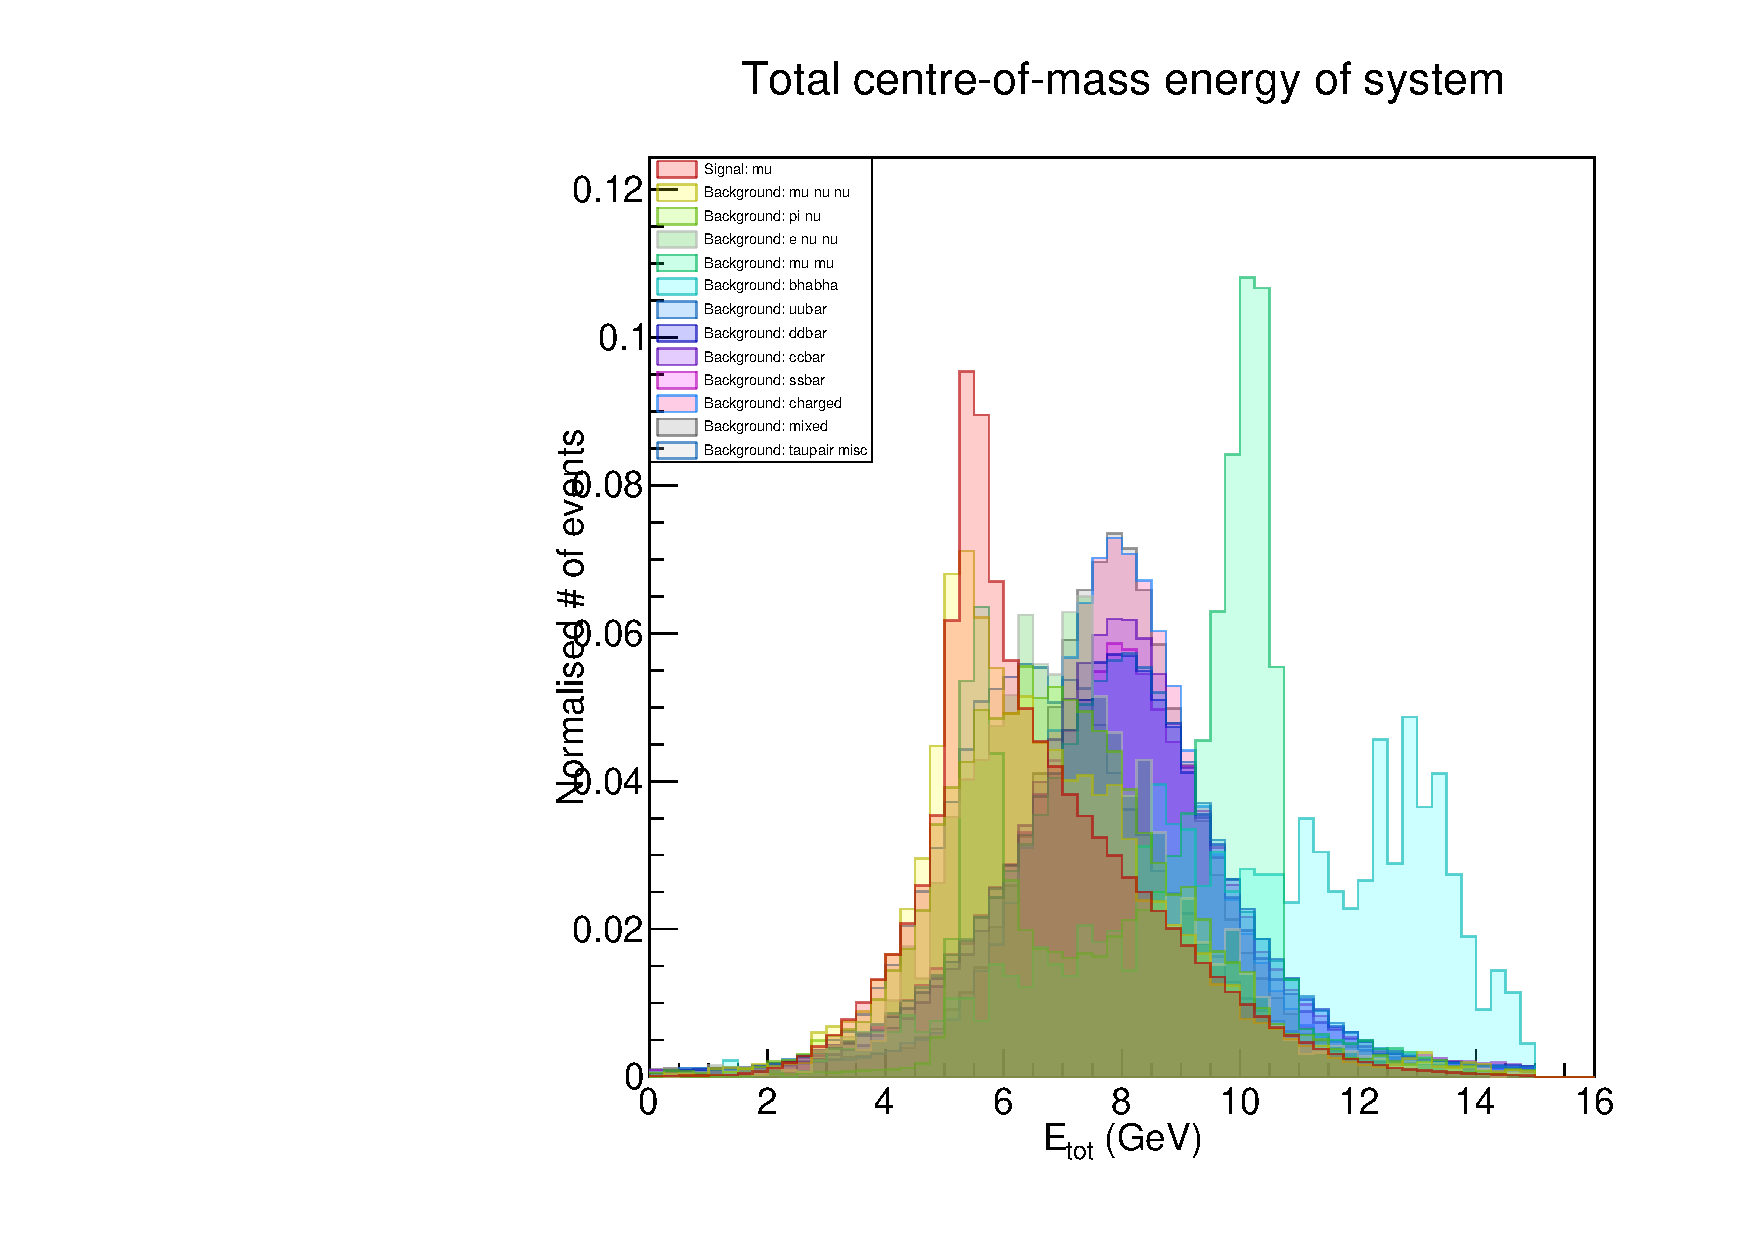
\includegraphics[width=\linewidth]{images/stack/stack_cut6_totalCM_E.pdf}
  \captionof{figure}{Another figure}
  \label{fig:test2}
\end{minipage}
\end{figure}

\begin{table}[h]
\centering
\begin{tabular}{llll}
\textbf{symbolic} & \textbf{description} & \textbf{lower} & \textbf{upper} \\ \hline
$p_{\text{tag}}^{\text{CM}}$  & CM momentum of tag track & --- & $\SI{5.2}{GeV}$ \\
$\cos\theta_{\text{signal}}$ & Cosine of polar angle of signal track & $-0.9$ & --- \\
$E_{\text{total}}^{\text{CM}}$ & Center-of-mass energy of total system  & --- & $\SI{15}{GeV}$ \\
$\lvert\text{thrust}\rvert$ & Magnitude of signal thrust vector* & 0.92 & --- \\
$E_{\text{sum}}^{\text{CM}}$ & Center-of-mass energy of photons and tracks & $\SI{4.5}{GeV}$ & ---
\end{tabular}
\caption{Preselection cuts (muon mode)}
\label{my-label}
\end{table}

Signal and background efficiencies after preselection are shown in Table ???? below.

\begin{table}[h]
\centering
\begin{tabular}{llll}
\textbf{MCtype} & \textbf{events in (reconstructed)} & \textbf{events out(preselection)} & $\mathbf{\epsilon_{\text{ps}}}$\\ \hline
\rowcolor[HTML]{EFEFEF}
$\tau\to\mu\gamma$ & 2914095 & 2857577 & 98.06\%	\\
\rowcolor[HTML]{EFEFEF}
$\tau\to e\gamma$ & 3111190 & 129863 & 4.17\%	\\
$\tau\to\mu\nu\nu$ & \num{32d6} & 153730 & 0.48\%\\
$\tau\to\pi\nu$ & \num{38d6} & 102813 & 0.27\%\\
$\tau\to e\nu\nu$ & \num{4.8d6} & 13322 & 0.28\%\\
$\tau\to\text{generic}$ & \num{63d6} & 47274 & 0.08\%\\
$e^+ e^-\to\mu^+\mu^-(\gamma)$ & \num{16.9332d6} & 8099760 & 47.83\%	\\
$e^+ e^-\to e^+e^-\gamma$ & \num{1.403d6} & 185377 & 13.21\%	\\
$e^+ e^-\to u\bar{u}$ & 20794 & 7352 & 35.36\%	\\
$e^+ e^-\to d\bar{d}$ & 20199 & 7259 & 35.94\%	\\
$e^+ e^-\to c\bar{c}$ & 13688 & 2424 & 17.71\%	\\
$e^+ e^-\to s\bar{s}$ & 15979 & 4856 & 30.39\%	\\
$e^+ e^-\to B^+B^-$ & 24907 & 3636 & 14.60\%	\\
$e^+ e^-\to B^0 \bar{B}^0$ & 26058 & 3550 & 13.62\%
\end{tabular}
\caption{Preselection efficiency (muon mode)}
\label{my-label}
\end{table}

\subsection{Electron mode}




Separate preselection criteria was chosen for the electron mode. 


\begin{figure}[h]
\centering
\begin{minipage}{.5\textwidth}
  \centering
  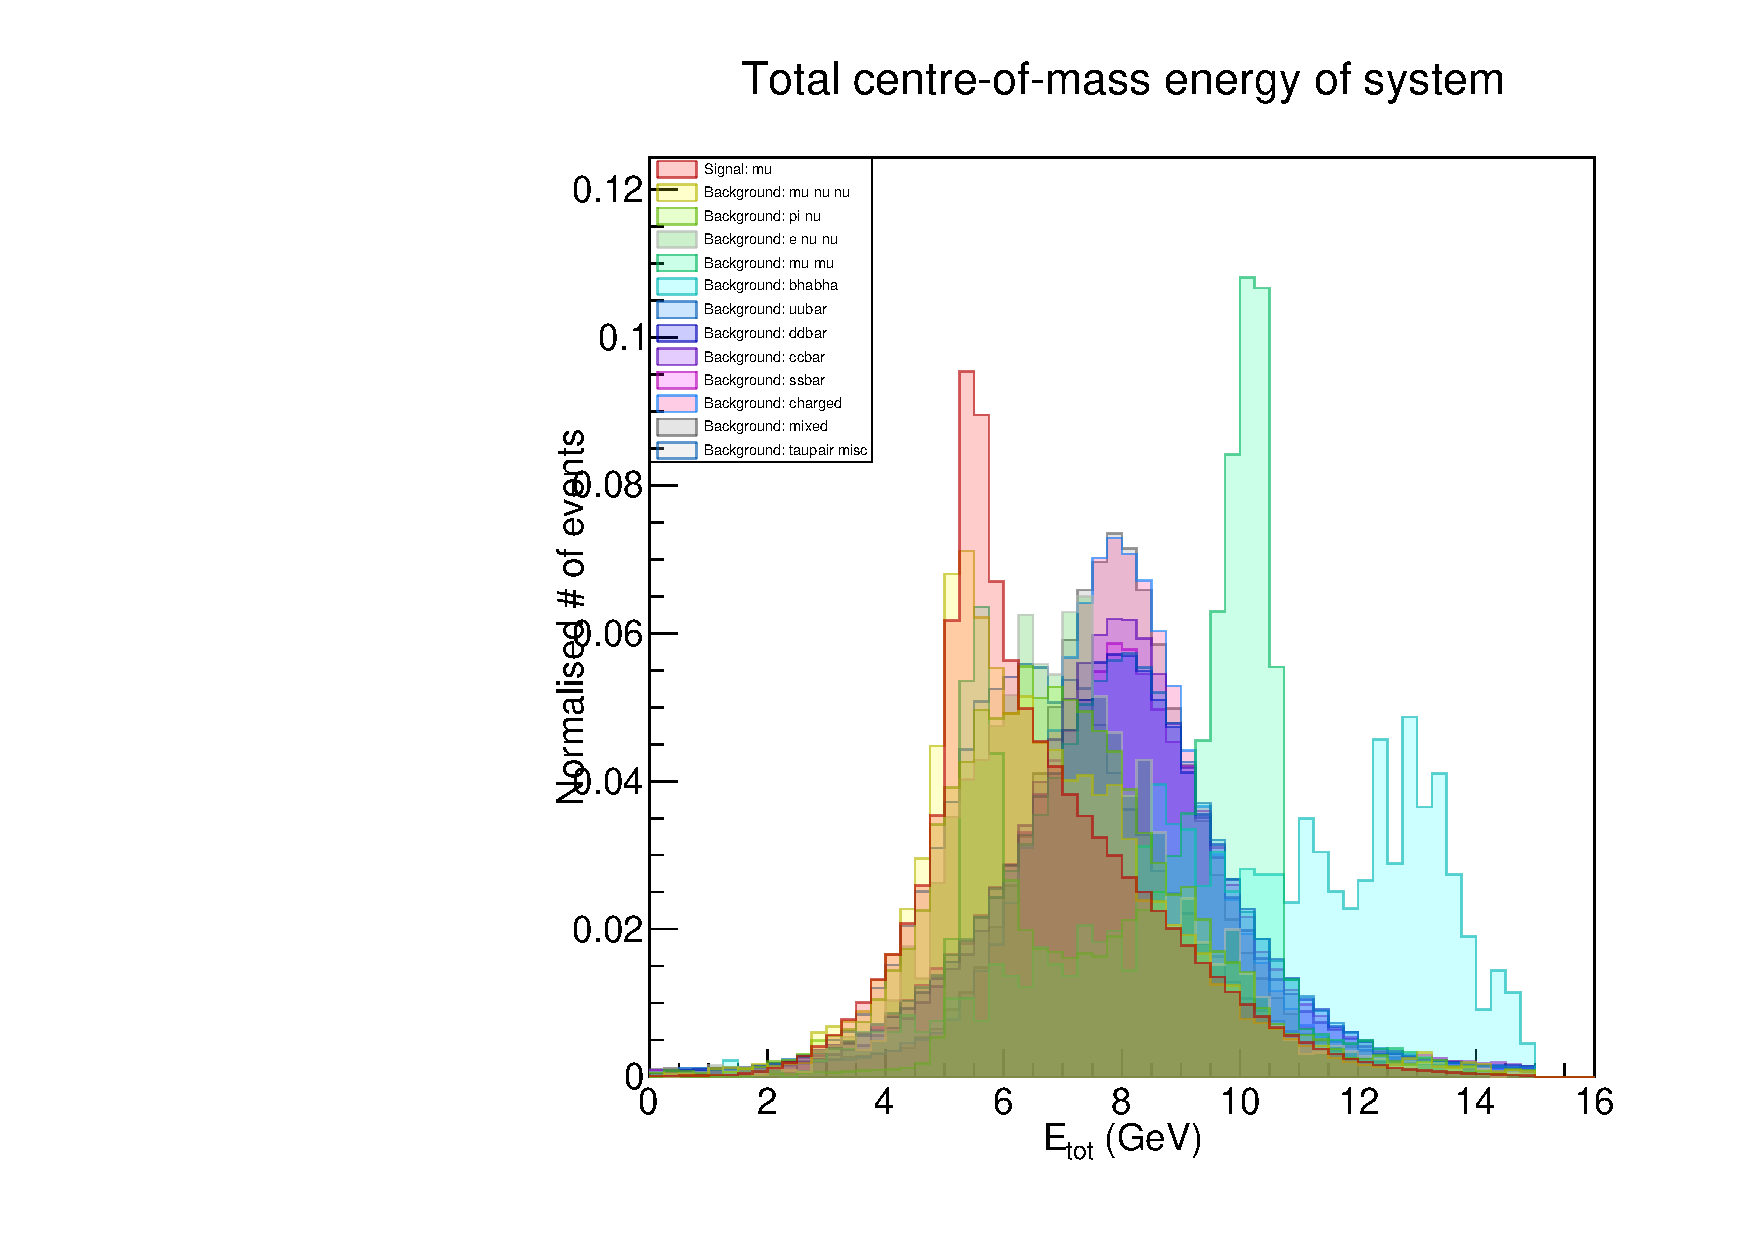
\includegraphics[width=\linewidth]{images/stack/stack_cut6_totalCM_E.pdf}
  \captionof{figure}{A figure}
  \label{fig:test1}
\end{minipage}%
\begin{minipage}{.5\textwidth}
  \centering
  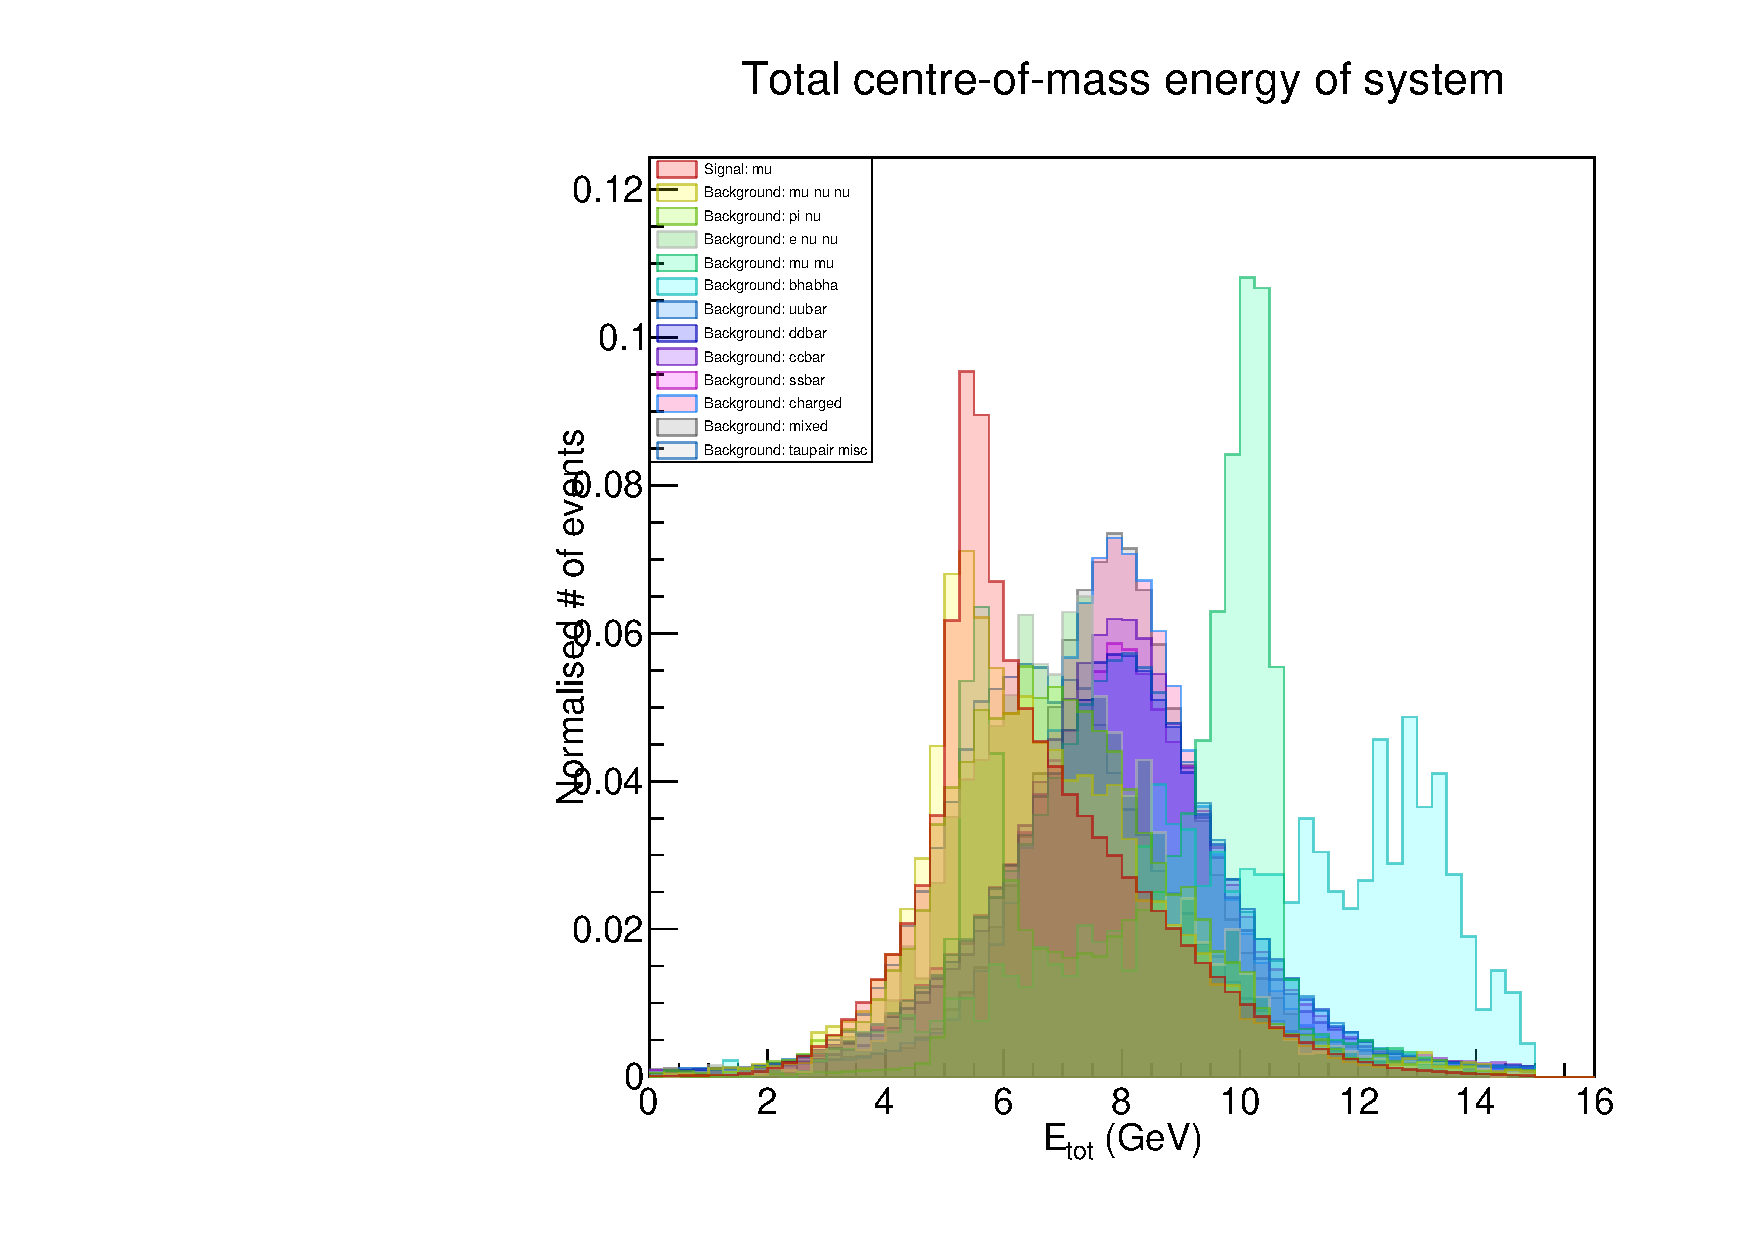
\includegraphics[width=\linewidth]{images/stack/stack_cut6_totalCM_E.pdf}
  \captionof{figure}{Another figure}
  \label{fig:test2}
\end{minipage}
\end{figure}

\begin{table}[h]
\centering
\begin{tabular}{llll}
\textbf{symbolic} & \textbf{description} & \textbf{lower} & \textbf{upper} \\ \hline
$p_{\text{tag}}^{\text{CM}}$  & CM momentum of tag track & --- & $\SI{5}{GeV}$ \\
$\cos\theta_{\text{signal}}$ & Cosine of polar angle of signal track & $-0.975$ & --- \\
$E_{\text{total}}^{\text{CM}}$ & Center-of-mass energy of total system  & --- & $\SI{15}{GeV}$ \\
$\lvert\text{thrust}\rvert$ & Magnitude of signal thrust vector* & 0.92 & --- \\
$E_{\text{sum}}^{\text{CM}}$ & Center-of-mass energy of photons and tracks & $\SI{4.5}{GeV}$ & ---
\end{tabular}
\caption{Preselection cuts (electron mode)}
\label{my-label}
\end{table}


``Bremmstrahlung.'' - Andrew, 2016.


\pagebreak

%-------------------------------------------------------------------

\section{Correlation}

The final signal region in which events will be selected from lies in $\Delta E$ vs. $M_{\text{inv}}$ space. To avoid biasing event selection, only loose cuts are applied to these variables throughout. We also investigate the correlation between these signal variables and other variables which we may cut over, to avoid introducing bias through these correlations. 

???

\pagebreak

%-------------------------------------------------------------------

\section{Scalings and signal optimisation}

The full Belle dataset has a time-integrated luminosity of $\SI{1000}{fb^{-1}}$. Instead of running over the equivalent amount of background events which we would expect in such a sample size, we can run over a smaller number of events then scale our results. WHY DO WE DO THIS?


After removing the most obvious background events from the analysis, the next step is to optimise signal efficiency. The measure of this ``optimisation'' is done maximising $S/\sqrt{S+B}$, where $S$ is the scaled number of signal events after selection, and $B$ is the scaled number of background events after selection.

Since each MC type uses a different number of generated events, the absolute number of events remaining is not a particularly useful number. Instead, we scale these events up (or down) to the number expected in a $\SI{1000}{fb^{-1}}$ data set – this is the total integrated luminosity available at Belle.

The scale factor for each MC type is calculated by

\begin{equation}
n_{\SI{1000}{fb^{-1}}} = n_{\text{generated}} \times \text{scale factor},
\end{equation}

where $n_{\SI{1000}{fb^{-1}}}$ = $\mathcal{L} \sigma$, and $n_{\text{generated}}$ is the number of events over which reconstruction is run. Expected number of events are compared below.


\begin{table}[h]
\centering
\begin{tabular}{lllll}
\textbf{MCtype} & $\mathbf{n_{\text{generated}}}$ & $\mathbf{n_{\SI{1000}{fb^{-1}}}}$ & 
\textbf{scale factor}\\\hline
\rowcolor[HTML]{EFEFEF} 
$\tau \to \mu\gamma$ & \num{3.1d6} & 82.71 & \num{2.66806d-5}\\
\rowcolor[HTML]{EFEFEF} 
$\tau \to e\gamma$ & \num{3.55d6} & 220.56 & \num{6.21296d-5} \\       
$\tau \to \mu\nu\nu$ & ?? & \num{3.19996d8} & 9.99987\\
$\tau \to \pi\nu$ & \num{38d6} & \num{1.99055d8} & 5.2383 \\
$\tau \to e\nu\nu$ & ?? & \num{3.27715d8} & 68.274 \\
$\tau \to \text{generic}$ & ?? & ?? & 15.7339  \\
$e^+e^- \to \mu^+\mu^-(\gamma)$ & \num{681d6} & \num{1.148d9} & 1.68576 \\
$e^+e^- \to e^+e^-\gamma$ & \num{71.52d6} & \num{3d11} & 4194.63 \\
$e^+e^- \to u\bar{u}$ & \num{d6} & \num{1.61d9} & 1610 \\
$e^+e^- \to d\bar{d}$ & \num{d6} & \num{4d8} & 400 \\
$e^+e^- \to c\bar{c}$ & \num{d6} & \num{1.3d9} & 1300 \\
$e^+e^- \to s\bar{s}$ & \num{d6} & \num{3.8d8} & 380 \\
$e^+e^- \to B^+B^-$ & \num{d6} & \num{1.2d9} & 1200 \\
$e^+e^- \to B^0\bar{B}^0$ & \num{d6} & \num{1.2d9} & 1200
\end{tabular}
\caption{Reconstruction efficiency}
\label{my-label}
\end{table}

A total of XXXX selection cuts were performed.

In optimizing the selection cuts, two distinct methods were used. In the first method, selection cuts were manually chosen based on a combination of individual threshold efficiencies and visual inspection. For individual threshold efficiencies, each cut was performed over all MC types with no other cuts, and the cut ``threshold'' varied each time. The output files were then used to produce figure-of-merit plots, where $S/\sqrt{S+B}$ was plotted against threshold; see below for a few examples. Cuts were applied in ``groups'', with more immediately clear cuts being performed first to reduce background for later cuts. After all cuts were performed, the signal and background efficiencies were as below, with the expected number of events.

EFFICIENCIES

The second method used multivariate analysis (MVA) methods, available through the Toolkit for Multivariate Analysis (TMVA). ??? haven't actually done this yet.

\begin{table}[h]
\centering
\begin{tabular}{lllll}
\textbf{cut number} & \textbf{symbolic} & \textbf{description} & \textbf{lower} & \textbf{upper} \\ \hline
\textbf{muCM\_P} & $p_{\text{signal}}^{\text{CM}}$  & CM momentum of signal track  &  &  \\
\textbf{tagtrackCM\_P} & $p_{\text{tag}}^{\text{CM}}$  & CM momentum of tag track &  &  \\
\textbf{mu\_Pt} & $p_{t~\text{signal}}$ & Transverse momentum of signal track &  &  \\
\textbf{mu\_Pt} & $p_{t~\text{tag}}$ & Transverse momentum of tag track &  &  \\
\textbf{muCosTheta} & $\cos\theta_{\text{signal}}$ & Cosine of polar angle of signal track &  &  \\
\textbf{tagtrackCosTheta} & $\cos\theta_{\text{tag}}$ & Cosine of polar angle of tag track &  &  \\
\textbf{totalCM\_E} & $E_{\text{total}}^{\text{CM}}$ & Center-of-mass energy of total system  &  &  \\
\textbf{thrustSignal} & $\lvert\text{thrust}_{\text{signal}}\rvert$ & Magnitude of signal thrust vector* &  &  \\
\textbf{signalPIDmu} & $\mu\text{-ID}_{\text{signal}}$ & $\mu$ PID of signal track &  &  \\
\textbf{mu\_P} & $p_{\text{signal}}$  & Momentum of signal track &  &  \\
\textbf{tagPIDmu} & $\mu\text{-ID}_{\text{tag}}$ & $\mu$ PID of tag track &  &  \\
\textbf{gamma\_E} & $E_{\gamma}$ & Energy of signal photon &  &  \\
 & $\cos\theta_{\gamma}$ & Cosine of polar angle of signal photon &  &  \\
 & $\cos\theta^{\text{CM}}_{\text{signal}-\gamma}$ & Cosine of angle between signal track and signal photon in CM &  &  \\
\textbf{sumCM\_E} & $E_{\text{sum}}^{\text{CM}}$ & Center-of-mass energy of photons and tracks &  &  \\
\textbf{tracksCMOpeningTheta} &  & Opening angle between signal and tag track &  &  \\
\textbf{helicityCosTheta} &  & Cosine of the helicity angle &  &  \\
\textbf{pmissing} & $p_{\text{miss}}$ & Missing momentum &  &  \\
\textbf{missingCosTheta} & $\cos\theta_{\text{miss}}$ & Cosine of polar angle of missing momentum vector &  &  \\
 & $\cos\theta^{\text{CM}}_{\text{miss-tag}}$ & Opening angle between tag track and missing momentum &  &  \\
\textbf{missingMassSqr} & $m_{\text{miss}}^2$ & Missing mass squared &  &  \\
\textbf{m\_nu2} & $m_{\nu}^2$ & Missing mass (tag side neutrino) squared &  &  \\
\textbf{tracks} & $n_{\text{tracks}}$ & Number of charged tracks &  &  \\
\textbf{signalPIDk} & $\text{K-ID}_{\text{signal}}$ & K PID of signal track &  &  \\
\textbf{signalPIDpi} & $\pi\text{-ID}_{\text{signal}}$ & $\pi$ PID of signal track &  &  \\
\textbf{signalPIDe} & $\text{e-ID}_{\text{signal}}$ & e PID of signal track &  &  \\
\textbf{clusterNHits} &  & timing of this cluster &  &  \\
\textbf{clusterUncorrE} &  & uncorrected cluster energy &  &  \\
\textbf{clusterHighE} &  & highest crystal energy in the cluster &  &  \\
\textbf{clusterTiming} &  & timing of this cluster &  &  \\
\textbf{signalTrPval} &  & Signal track fit pvalue &  &  \\
\textbf{tagTrPval} &  & Tag track fit pvalue &  &  \\
\textbf{cosTBz} &  & Cosine of the angle between the thrust axis of the signal track and the z-axis &  &  \\
\textbf{cc1} &  & Cleo cone 1 &  &  \\
\textbf{hso00} &  & Hso(0,0) &  &  \\
\textbf{neutralECLEnergy} &  & Total energy of all neutral ECLClusters &  & 
\end{tabular}
\caption{Selection criteria}
\label{my-label}
\end{table}

\emph{Note that these cluster based quantities apply to particles constructed from ECL clusters} (from NtupleTool page).


\pagebreak

%-------------------------------------------------------------------

\section{Signal region and event selection}

After selection, we are left with a far reduced number of background events and a non-neglible amount of expected signal events. We can now analyse events within the signal region. This is a region in $\Delta E$ vs $M_{\text{inv}}$ space, with $-0.2 < \Delta E < 0.2$, and $1.7 < M_{\text{inv}} < 1.8$.

$\Delta E$ is the energy difference between the reconstructed particles and beam energy, calculated as ????. $M_{\text{inv}}$ is the invariant mass of the reconstructed signal tau; experimentally the tau has a mass of $\SI{1.7}{GeV/c}$. These variables have only been cut on very loosely up until this point to avoid bias.

\pagebreak

%-------------------------------------------------------------------

\section{Conclusion}

\subsection{Future improvements}

\subsection{Working group status}

???

\subsection{Expected impact on Belle II}



%-----------------------------------------
\bibliographystyle{plain}
\bibliography{refs.bib}
\end{document}







